\documentclass[conference]{IEEEtran}
% todo change back, for now I need to read lol
% \documentclass{report}

\usepackage{cite}
\usepackage{graphicx}
\usepackage{amsmath}
\usepackage{algorithmic}
\usepackage[caption=false,font=normalsize,labelfont=sf,textfont=sf]{subfig}
\usepackage{url}
\usepackage{hyperref}
\usepackage{float}
\usepackage{listings}
% Customizing lstlisting to mimic verbatim
\lstset{
  basicstyle=\ttfamily,
  breaklines=true, % Allows line breaks
  postbreak=\mbox{\space}, % Optional: mark line breaks
  escapeinside={(@}{@)}, % Define escape characters
}

% correct bad hyphenation here
\hyphenation{op-tical net-works semi-conduc-tor}


\begin{document}
\title{Simulation and Performance Evaluation\\ Project}


% author names and affiliations
% use a multiple column layout for up to three different
% affiliations
\author{\IEEEauthorblockN{Manuela Corte Pause}
  \IEEEauthorblockA{manuela.cortepause@studenti.unitn.it
    \\240183}
  \and
  \IEEEauthorblockN{Simone Marrocco}
  \IEEEauthorblockA{simone.marrocco@studenti.unitn.it
    \\239951}
}

% make the title area
\maketitle

% As a general rule, do not put math, special symbols or citations
% in the abstract
\begin{abstract}
  The relationship between economic indicators is a topic on interest for economists and policy makers to improve the lives of the citizens. In this project, we explore the relationship between the Gross Domestic Product (GDP), the Inflation Rate (IR) and the Consumer Price Index (CPI). We first conduct a preliminary analysis of the correlation between the variables and then we try to explicitly model them using two different approaches: the Prais-Winsten Model and the Hidden Markov Model. We then use the models to predict the GDP for the next year and compare the results. We find that the Hidden Markov Model is able to capture the dynamics of the data better than the Prais-Winsten Model, but our simplified analysis restricted it to only predict whether the GDP will increase or decrease. The Pais-Winsten Model, on the other hand, is able to predict the GDP value for the next years, but is not as reliable.
\end{abstract}


% For peerreview papers, this IEEEtran command inserts a page break and
% creates the second title. It will be ignored for other modes.
\IEEEpeerreviewmaketitle


\section{INTRODUCTION}
In recent years, crisis like the COVID-19 pandemic and the war in Ukraine have severely limited the GDP growth of all nations, slowing down progress and making life for families and industries more difficult than ever.

Three main factors have increased inflation and the price of products: first, the global traffic of goods stopped because of the lock downs; then, the Russian sanctions increased the energy cost to produce them; finally, the recovery of the free trade increased demand.

To counter that, the current economic theory states that in order to decrease inflation central banks need to increase interest rates, in order to keep around 3\% the increase of prices. Too high money devaluation makes investments and currency useless, while too low devaluation creates economic stagnation. This policies are made to keep stable growth, measured in Gross Domestic Product (GDP).

But is this claim true? Is there really a correlation between GDP and inflation, and an inverse correlation between GDP and interest rate? In this short paper, our aim is to first find this correlation by looking at the economic figures history of some of the best economies in the world; then, if it exists, use it to make a prediction of the last years without the crises, to see how much they influenced negatively the well being of the world.

All code produced, as well as a copy of the paper, can be found on GitHub at \href{https://github.com/ManuelaCorte/SPE-Project}{https://github.com/ManuelaCorte/SPE-Project}.

\section{RELATED WORKS}
\label{sec:related_works}
The task of understanding and predicting the relationships between economic indicators has been the subject of many studies in the past. In this section, we will review some of the most relevant works in this field.

\subsection*{Economic Indicators}
\label{subsec:economic_indicators}
The Gross Domestic Product (GDP) is a measure of the economic performance of a country. It represents the total value of all goods and services produced in a country over a specific period of time. The GDP is considered to be one of the most important economic indicators, as it provides a comprehensive view of the overall health of an economy.

The other macroeconomic indicators that we will consider in our work are:
\begin{itemize}
  \item Interest Rate: The rate of interest measures the percentage reward a lender receives for deferring the consumption of resources until a future date. Correspondingly, it measures the price a borrower pays to have resources now.
  \item Consumer Price Index (CPI): The CPI is a measure of the prices of a representative basket of goods and services purchased by a typical household. It is considered to be a key indicator of inflation, as it reflects the cost of living for citizens.
\end{itemize}

Different approaches have been used to model the relationships between these economic indicators. For example, in \cite{gdp_early} a regression model is used to analyze the relationships between GDP, interest rates, exchange rates, and other market indicators such as Sensex. The authors find that inflation is highly correlated with GDP but does not have a significant impact on GDP growth while market indicators and exchange rates have a significant correlation with GDP.

Another study \cite{gdp_regr} uses a Partial Least Squares (PLS) model and path analysis with the intent of explaining direct and indirect relationships between GDP, interest rate, exchange rate, and inflation. Similarly to \cite{gdp_early}, the authors find that inflation has a limited impact on GDP, while the exchange rate has a positive correlation with GDP. As for the interest rate, it has a negative impact on GDP. It is also interesting to consider the relation between interest rates and inflation which are negatively correlated. This is to be expected as increasing interest rates is used as a tool to control inflation as describe in \cite{imf}.

\section{DATA}
\label{sec:data}

In this section we describe the data used for this analysis. We use data from the International Monetary Fund \href{https://www.imf.org/en/Data}{IMF} for the Gross Domestic Product (GDP) and the Interest Rates (IR) while the data about the Consumer Price Index was taken from the \href{https://www.worldbank.org/en/research/brief/inflation-database}{World Bank Group}. The data we were most interested in were the monthly values for our economics indicators to have a larger volume of data to use but we could only find quarterly data for the GDP. In order to have the same number of data points for all the indicators we decided to use linear interpolation to fill the missing values. The same procedure was similarly done for the Interest Rates as well but this only involved a few countries.

The data was then divided in three sections: training, test and COVID. The training data was used to train the models and contained all data up to the end of 2016. The test data was used to test the models and contained all data from the beginning of 2017 to the end of 2019. The COVID data was used to test the models in the presence of a situation outside the situation in which the models were trained and contained all data from the beginning of 2020 to the end of the available data. Moreover, the GDP data was expressed in hundred million dollars to have more manageable orders of magnitude.

After this preliminary analysis all countries that didn't have one of the indicators were removed. For data that either didn't have data for the test or COVID period, they were used differently depending on the model. For the initial correlation analysis we used all data available, for the Hidden Markov Model the data was used to train the model but it is not possible to test the model on the specific country. For the regression model, the countries that didn't have data for the test period where not considered viable for the analysis.

Overall, this leaves us with 25 countries for the correlation analysis and the Hidden Markov Model and 13 countries for the regression: Brazil, India, Indonesia, Italy, Israel, Mexico, Norway, Russia, South Africa, Switzerland, South Korea, Ukraine and United States.

\section{CORRELATION}
As stated before, we are interested in the correlation between Interest Rates, Consumer Price Index and Gross Domestic Product in order to understand if the current economic theory of increasing interest rate to control inflation and maintaining a healthy economy is true. As a first step, to this analysis we conduct a correlation analysis between the three variables. In order to achieve more reliable results without making any assumptions about the distribution of the data, we calculate the correlation coefficients using bootstrapping.

\subsection*{Statistical Background}
There are many ways to measure the correlation between two variables. The most common method is the Pearson correlation coefficient which is a measure of linear correlation between two variable $X$ and $Y$.
\begin{equation*}
    \rho_{X,Y} = \frac{cov(X,Y)}{\sigma_X \sigma_Y} = \frac{E[(X-\mu_X)(Y-\mu_Y)]}{\sigma_X \sigma_Y}
\end{equation*}
The Pearson correlation coefficient is a value between -1 and 1 where 1 means that the two variables are perfectly correlated, 0 means that there is no correlation and -1 means that the two variables are perfectly negative-correlated.

More options are available to measure the correlation between two variable. For example, the Spearman's rank correlation coefficient is a measure of monotonic correlation, whether linear or not. It is equivalent to the Pearson correlation coefficient of the rank variables where the rank of a variable is the position the variable would have if the data were sorted in ascending order.
\begin{align*}
    \rho_{X,Y} & = 1 - \frac{6 \sum d_i^2}{n(n^2-1)} \\
    d_i        & = rank(X_i) - rank(Y_i)
\end{align*}
where $d_i$ is the difference between the ranks of the two variables for the $i$-th observation.

It is important to remember that more complex relationships can exist between variables that neither the Pearson nor the Spearman correlation coefficient can capture (e.g. quadratic relationships).

Another measure of rank correlation is the Kendall's tau coefficient which is a measure of the correspondence between the rankings of two variables:
\begin{align*}
    \tau = \frac{P-Q}{\frac{1}{2}n(n-1)} \\
\end{align*}
where $P$ is the number of concordant pairs and $Q$ is the number of discordant pairs. A pair of observations $(x_{i},y_{i})$ and $( x_j , y_j) $ is said to be concordant if the sort order of $( x_i , x_j )$ and $( y_i , y_j )$ agrees: that is, if either both  $x_{i}>x_{j}$ and  $y_{i}>y_{j}$ or both $\displaystyle x_{i}<x_{j}$ and $y_{i}<y_{j}$ holds.

Because they deal with with rank variables instead of raw data, the Spearman and Kendall coefficients are less sensitive to outliers than the Pearson coefficient.

\subsection*{Results}
In figure \ref{fig:correlation_italy} we show the correlation between Interest Rates, Consumer Price Index and Gross Domestic Product for Italy. The correlation coefficients are calculated using bootstrapping with 1000 repetitions. The confidence intervals are calculated using the percentile method with a confidence level of 95\%.
As we can see in \ref{fig:correlation_italy}, the correlation between Interest Rates and Consumer Price Index is strongly negative, while the correlation between Interest Rates and Gross Domestic Product is weakly negative as we expected.

\begin{figure}[H]
    \centering
    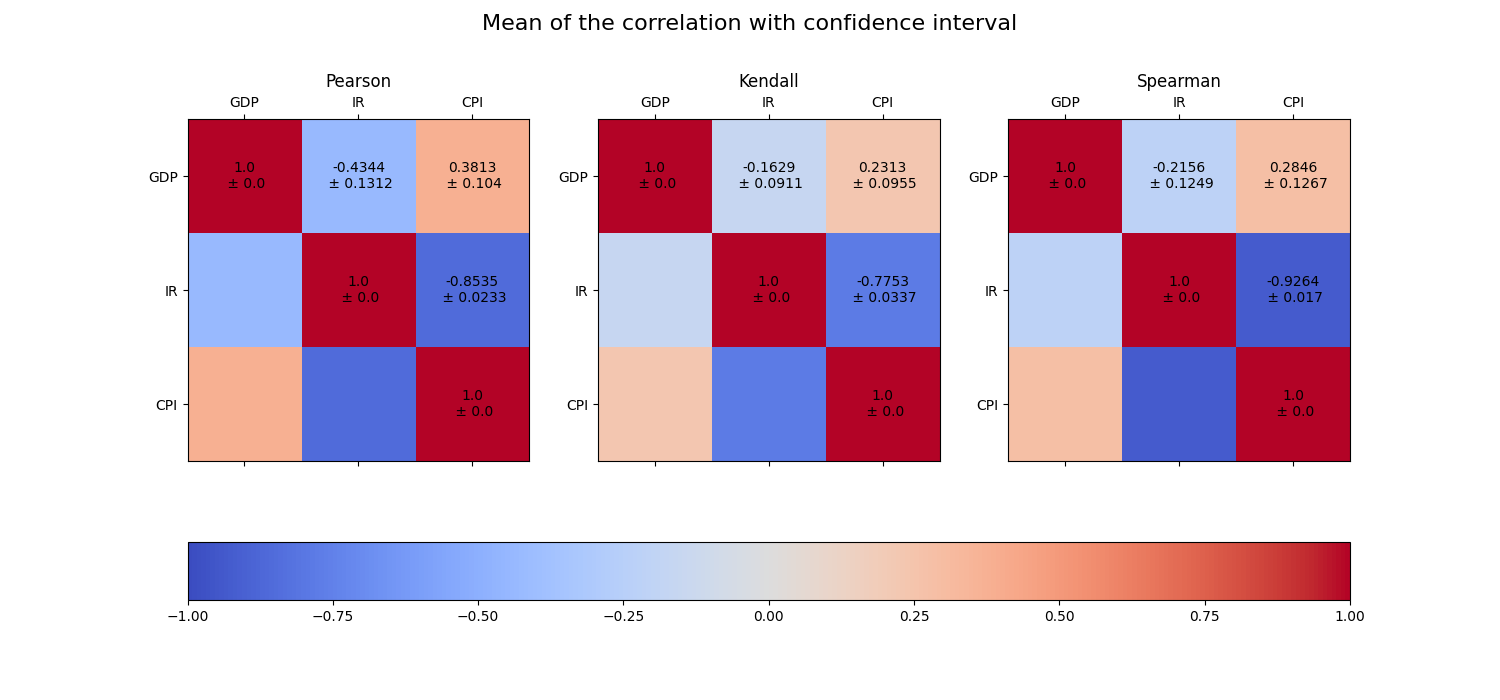
\includegraphics[width=\linewidth]{imgs/italy_correlation.png}
    \caption{Correlation between Interest Rates, Consumer Price Index and Gross Domestic Product of Italy}
    \label{fig:correlation_italy}
\end{figure}

For other countries, for example the United States (figure \ref{fig:correlation_us}), both the correlation between Interest Rates and Consumer Price Index and the correlation between Interest Rates and Gross Domestic Product are stronger than for Italy. This could be caused by the strong and self sufficient economy of the USA: being less dependant on other conditions like international trading, other countries crisis or slow growth, and being the central economic power of the world, the monetary policies of the Federal Reserve (the american Central Bank) have more impact on the internal economy.

\begin{figure}[H]
    \centering
    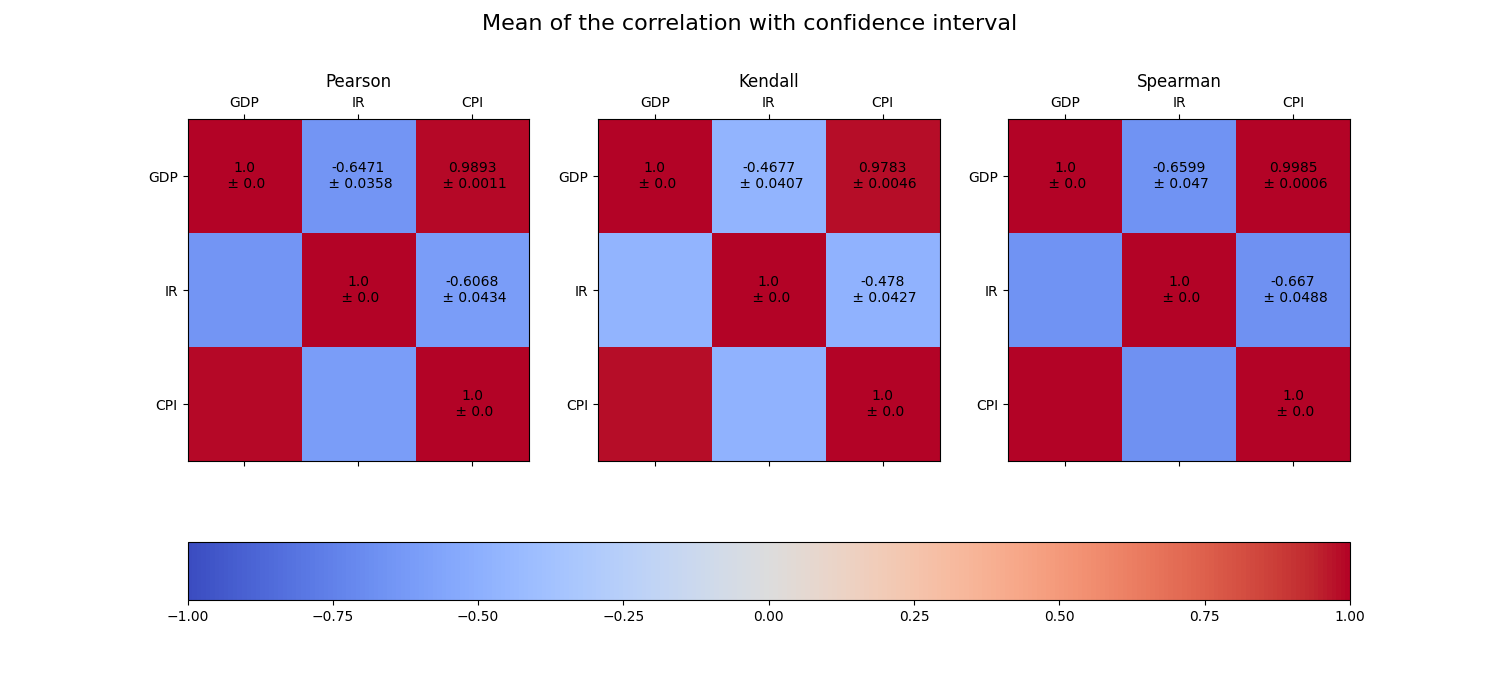
\includegraphics[width=\linewidth]{imgs/usa_correlation.png}
    \caption{Correlation between Interest Rates, Consumer Price Index and Gross Domestic Product of the United States of America}
    \label{fig:correlation_us}
\end{figure}

We also analyze the overall relationships by putting together the data for all countries in figure \ref{fig:correlation_global}. We can observe that the correlation between Interest Rates and Consumer Prince Index remains negative albeit weaker than for the individual countries above while the correlation between Interest Rates and Gross Domestic Product is very weakly positive. This could be due to the fact that economies have different conditions and responses to economic stimulus. Our analysis is also simplified and does not consider steps of increases, putting as the same an inflation of 3\%, which is good according to the current economic theory, and 20\%, which is too high and dangerous.

\begin{figure}[H]
    \centering
    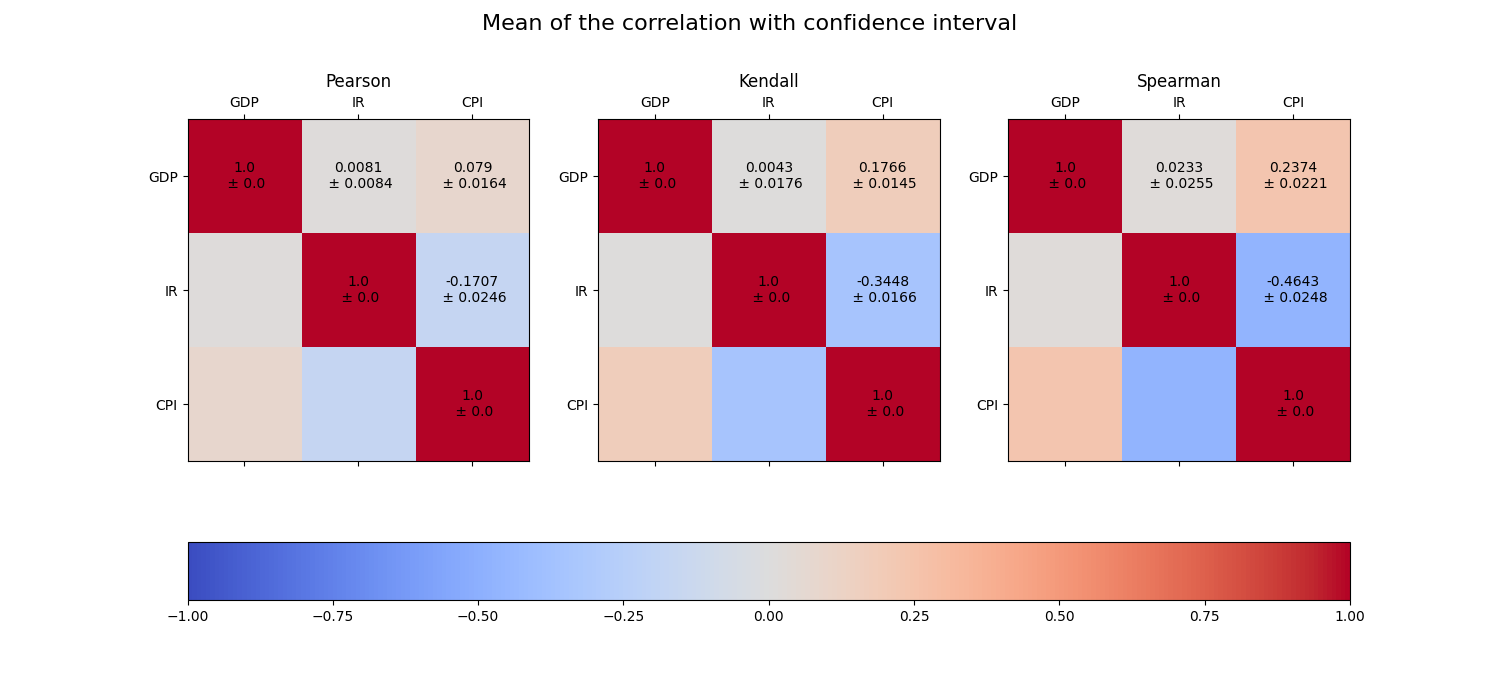
\includegraphics[width=\linewidth]{imgs/all_countries_correlation.png}
    \caption{Correlation between Interest Rates, Consumer Price Index and Gross Domestic Product of all economies studied combined}
    \label{fig:correlation_global}
\end{figure}

This first analysis shows us that the correlation between the three variable is not entirely as we expected. This could be due to the fact that the relationship between the variables is very complex and cannot be captured by simple linear or monotonic correlation coefficients.

\section{PRAIS-WINSTEN ESTIMATION}
\label{sec:regression}
As we imagine there is a correlation between Interest Rate, Inflation and Gross Domestic Product, then we could ask: is there a way to model how changes in the first two variables affect the third, and can we predict how a country could change from a situation to another? We try to answer these questions in the following sections.

\subsection*{Statistical Background}
Ordinary Least Squares(OLS) is a widely used method for estimating the parameters of a linear regression model. However, OLS has some limitations, such as the assumption of homoscedasticity and the independence of the residuals. When these assumptions are violated, the estimates are biased and the standard errors are not reliable. Time series data often violates these assumptions, as the observation are not independent and the residuals are autocorrelated. There are several methods to deal with these issues, both with models specific for time series such as ARIMA models and with models that try to fix the data before applying OLS. One of these models is the Prais-Winsten Estimator \cite{prais}, which is a method to correct the OLS estimates by assuming the residuals are autocorrelated.

Consider the linear regression model
\begin{align*}
  y_t = \alpha + \beta x_t + \epsilon_t
\end{align*}
where we assume the residuals $\epsilon_t$ can be modelled as a first order autoregressive process $AR(1)$ $\epsilon_t = \rho \epsilon_{t-1} + e_t, |\rho|<1$. The Prais-Winsten Estimator is then obtained by applying the following transformation to the data:
\begin{align*}
  y_{t}-\rho y_{t-1}         & =\alpha (1-\rho )+(X_{t}-\rho X_{t-1})\beta + e_{t}                                                               \\\\
  {\sqrt {1-\rho ^{2}}}y_{1} & =\alpha {\sqrt {1-\rho ^{2}}}+\left({\sqrt {1-\rho ^{2}}}X_{1}\right)\beta +{\sqrt {1-\rho ^{2}}}\varepsilon _{1}
\end{align*}
This method is a modification of the Cochrane-Orcutt method \cite{cochrane}, but has the additional transformation for the first observation $y_1$ while the Cochrane-Orcutt method only transforms the data for $t>1$.

The Prais-Winsten Estimator is an iterative method, where we first estimate $\rho$ using the residuals of the OLS model and then apply the transformation to the data described above and fit a new OLS model until convergence. The convergence criteria can be based on the change in the estimates of $\rho$ or by statistical tests on the residuals such as the Ljung-Box test or the Durbin-Watson test.

Here we show the results of the Prais-Winsten Estimator on the data for Italy. As an introductory step, we show the time series for GDP, IR and CPI for Italy (Figure \ref{fig:italy_ts}).
\begin{figure}[H]
  \includegraphics[width=.9\linewidth]{imgs/italy_gdp.png}
  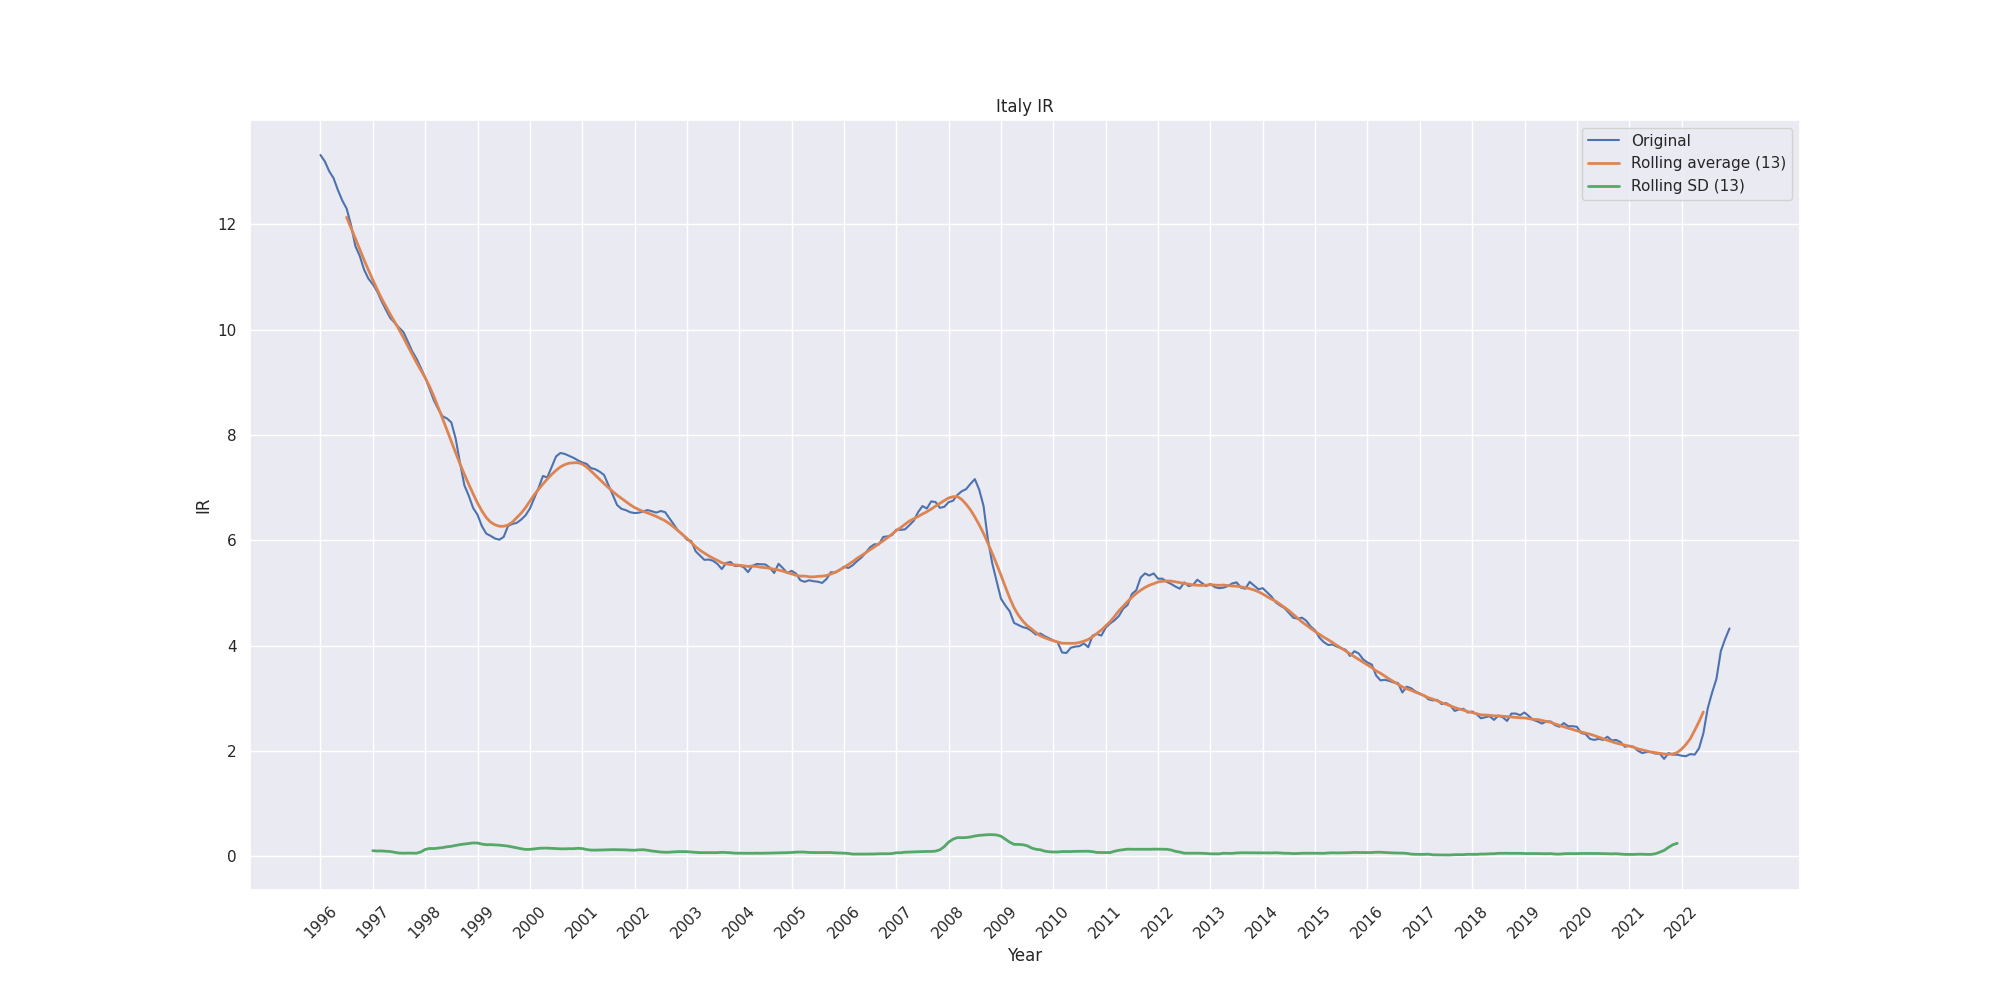
\includegraphics[width=.9\linewidth]{imgs/italy_ir.png}
  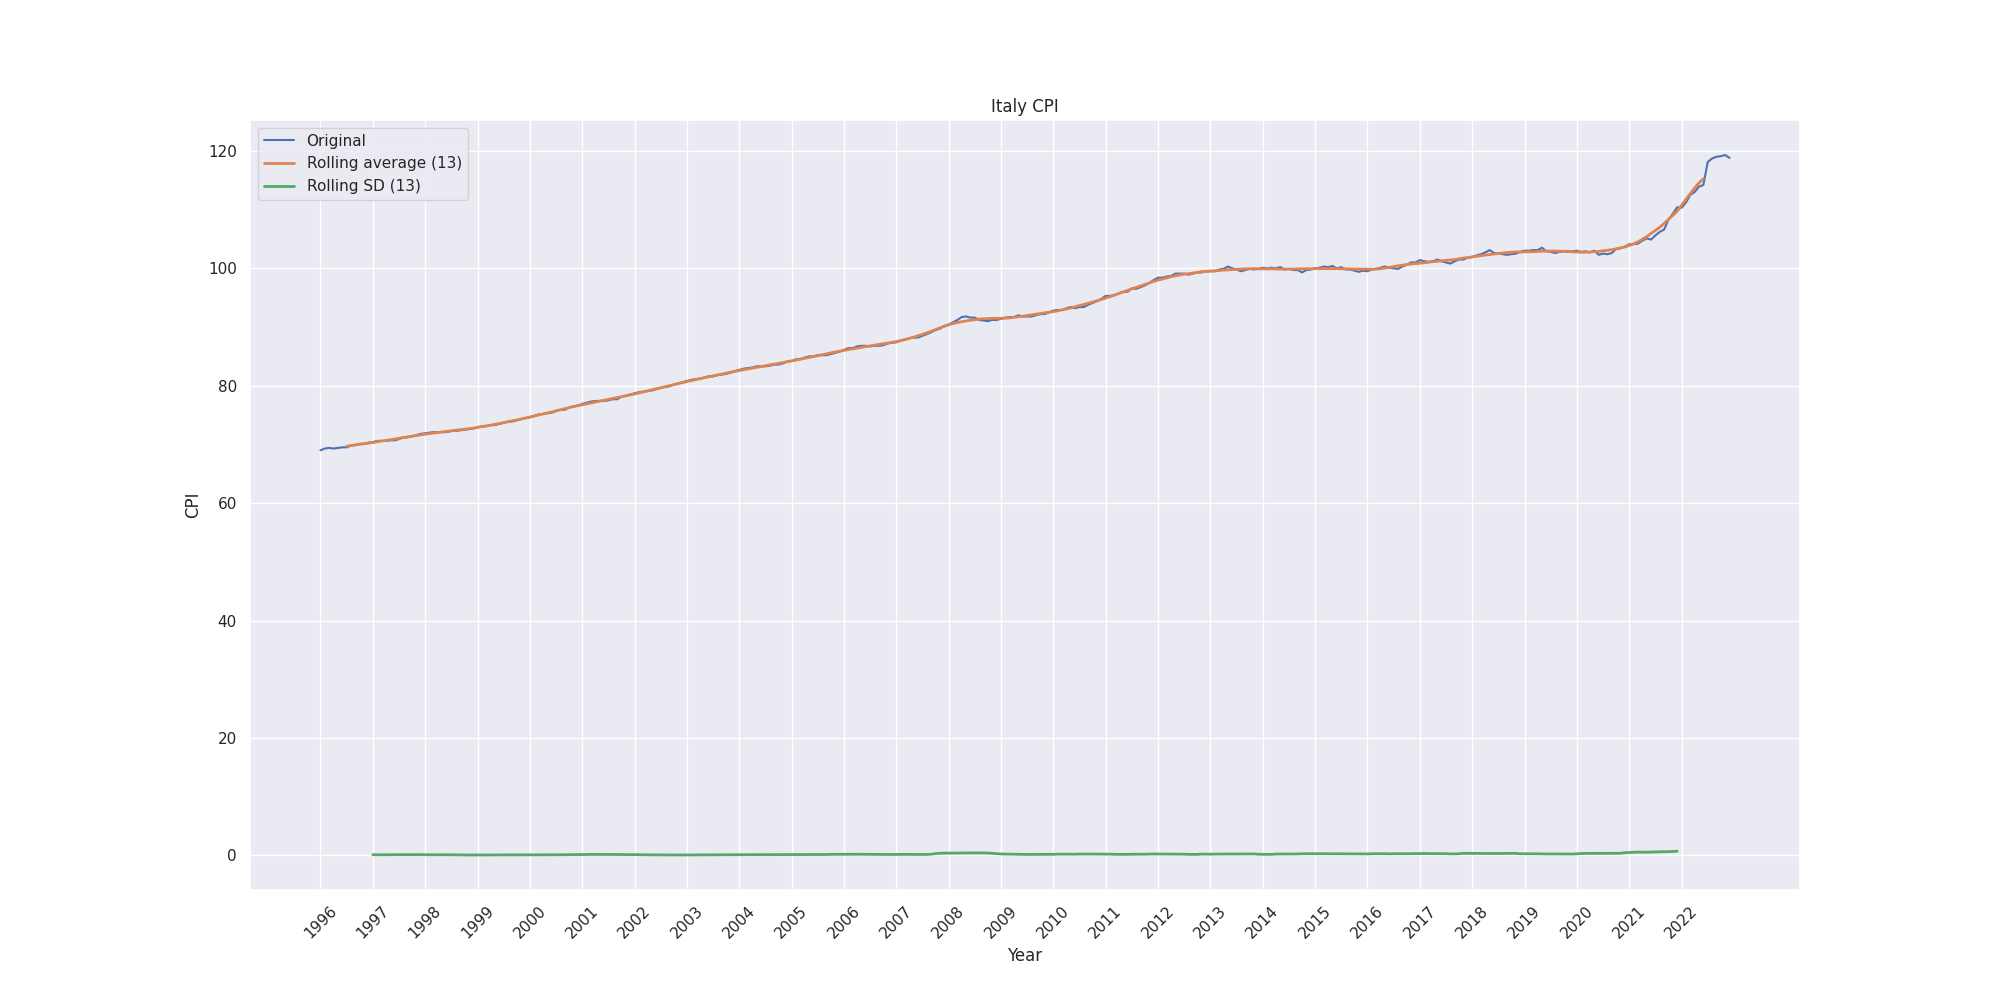
\includegraphics[width=.9\linewidth]{imgs/italy_cpi.png}
  \caption{Time series for Italy}
  \label{fig:italy_ts}
\end{figure}


We can see that the time series for GDP, IR and CPI are not stationary, so we first take the first differences (Figure \ref{fig:italy_diff}) which means we subtract the value at time $t-1$ from the value at time $t$. This transformation allows us to make data stationary and reduce autocorrelation.

\begin{figure}[H]
  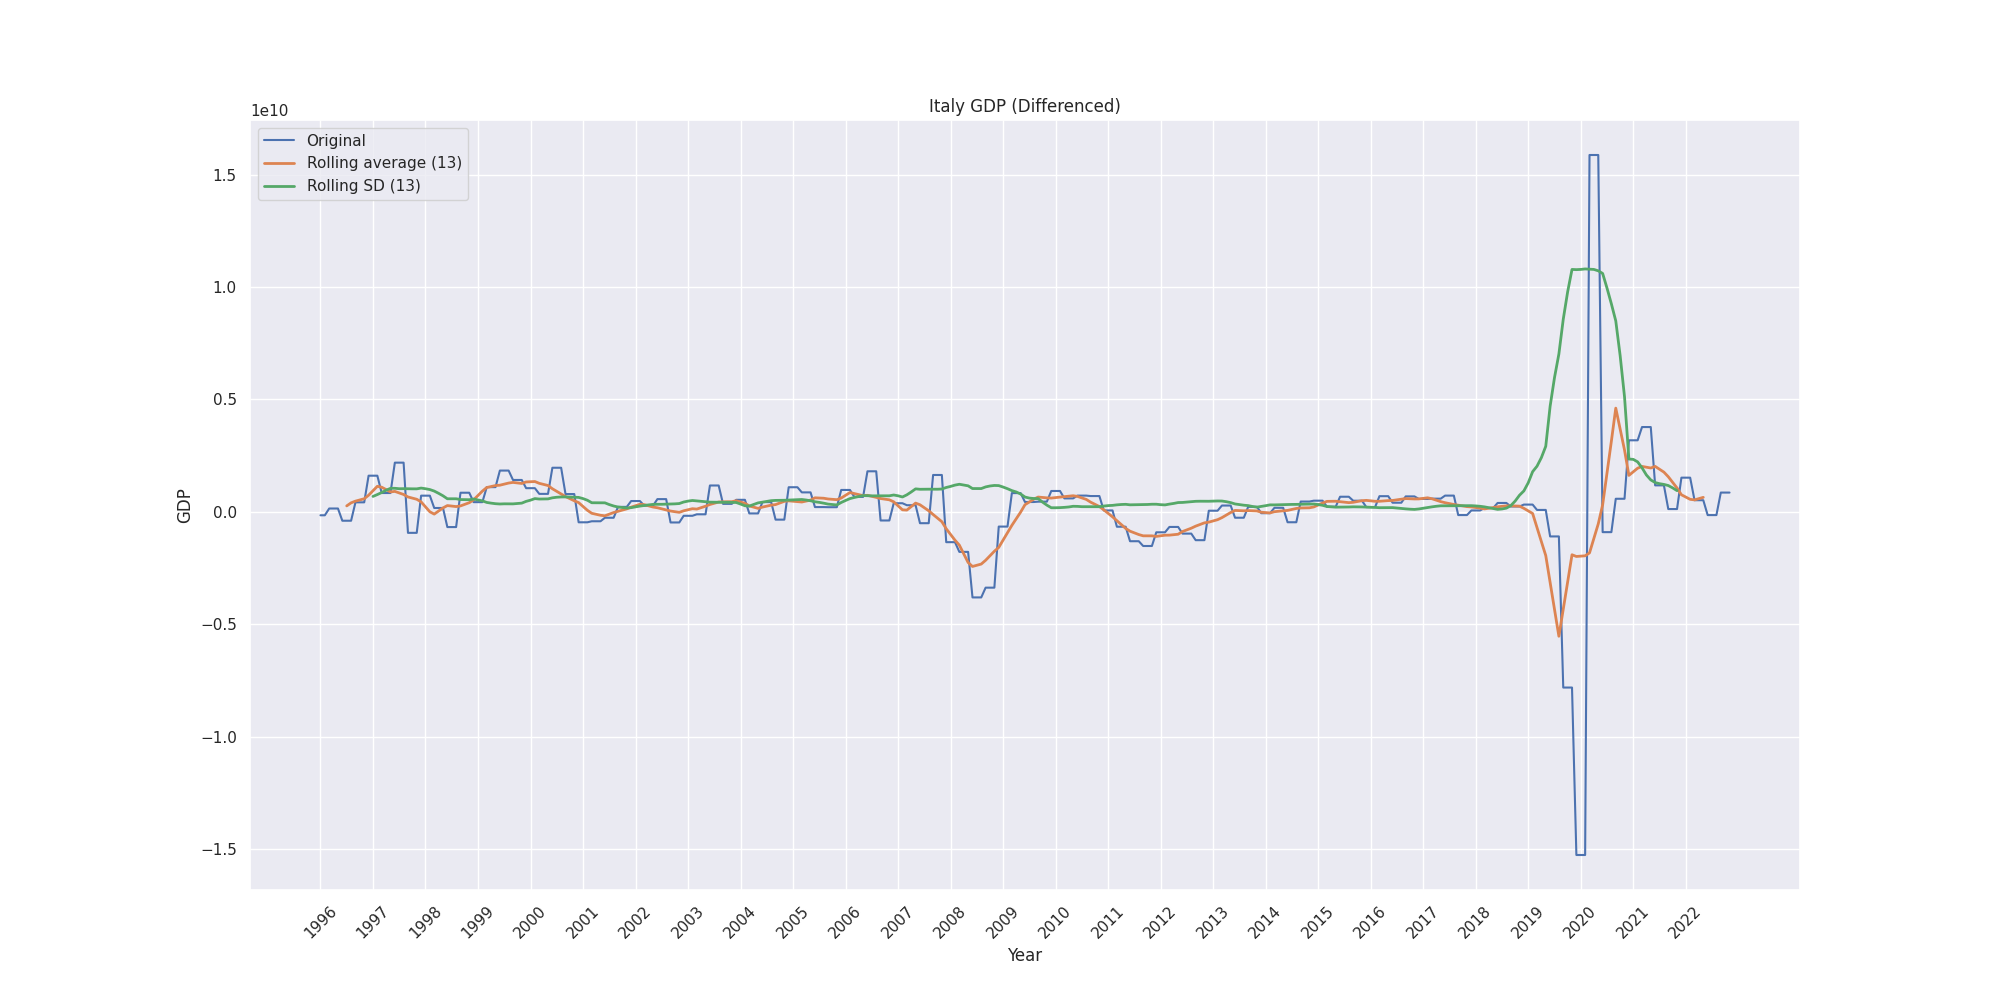
\includegraphics[width=.9\linewidth]{imgs/italy_gdp_diff.png}
  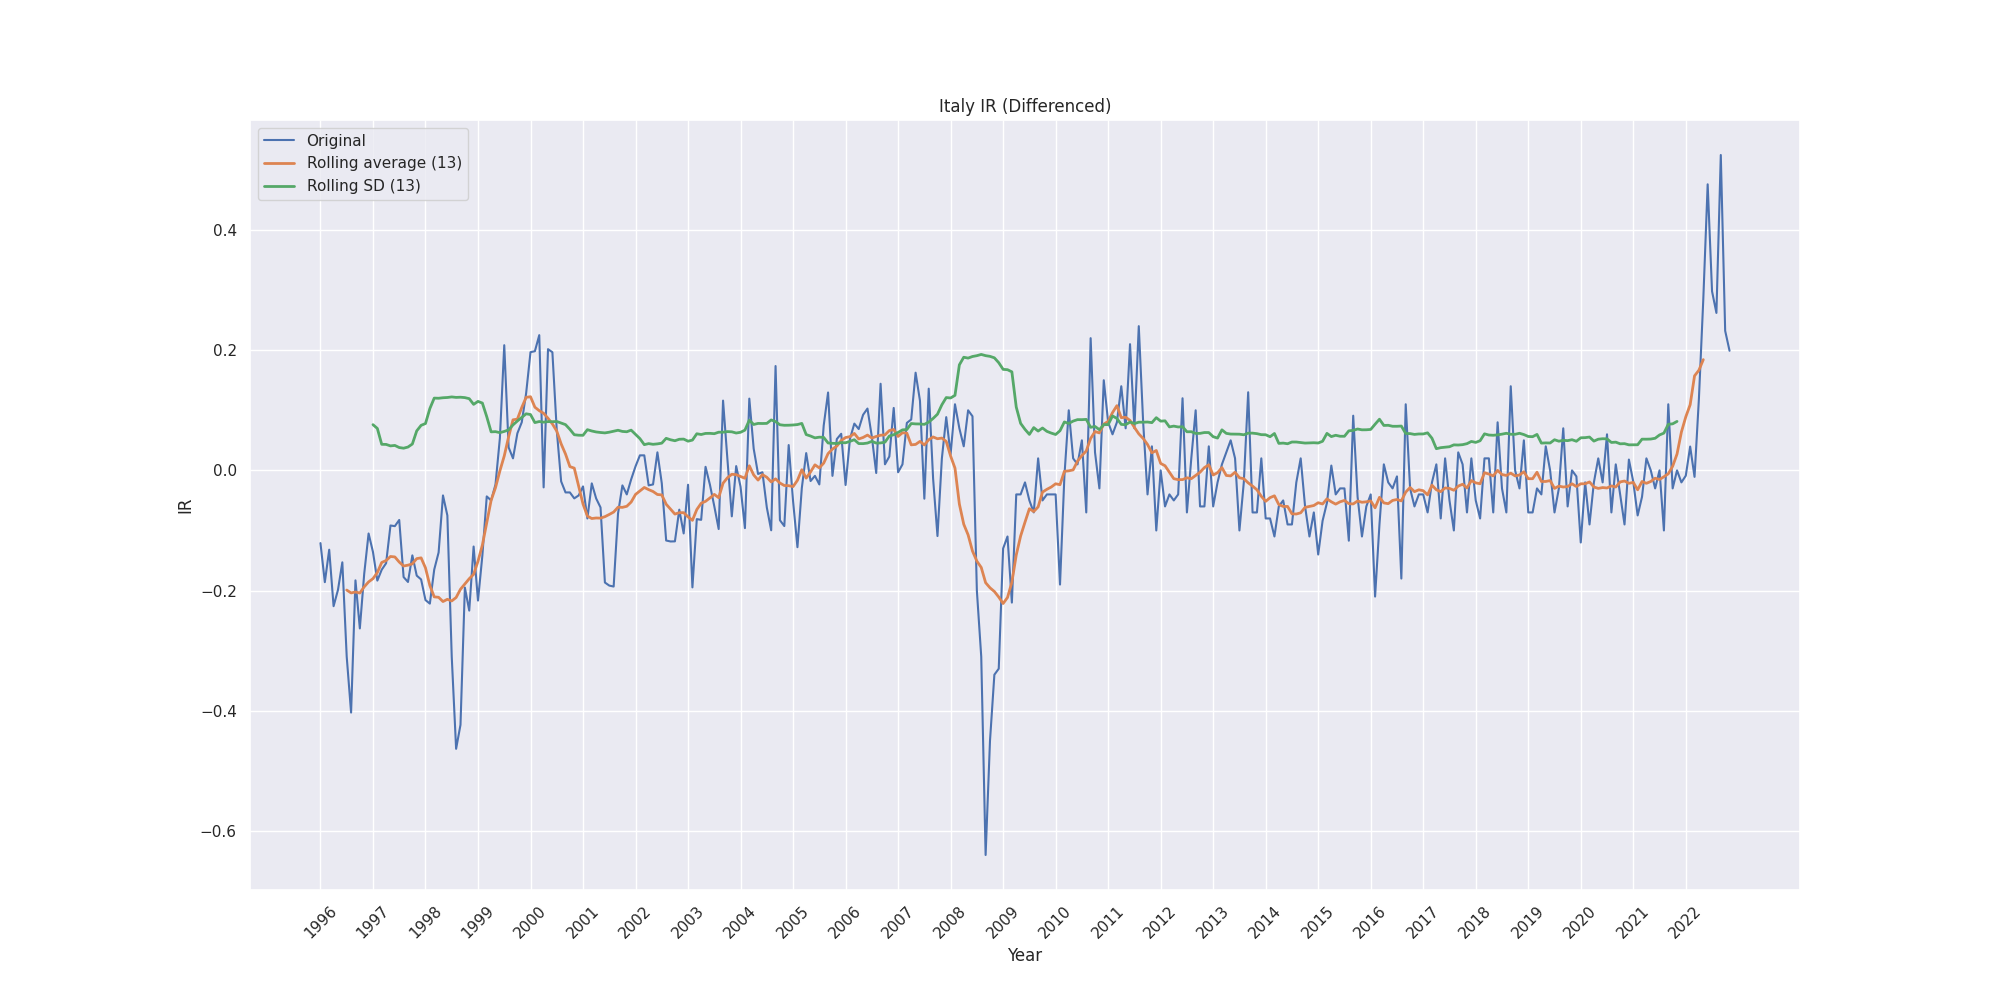
\includegraphics[width=.9\linewidth]{imgs/italy_ir_diff.png}
  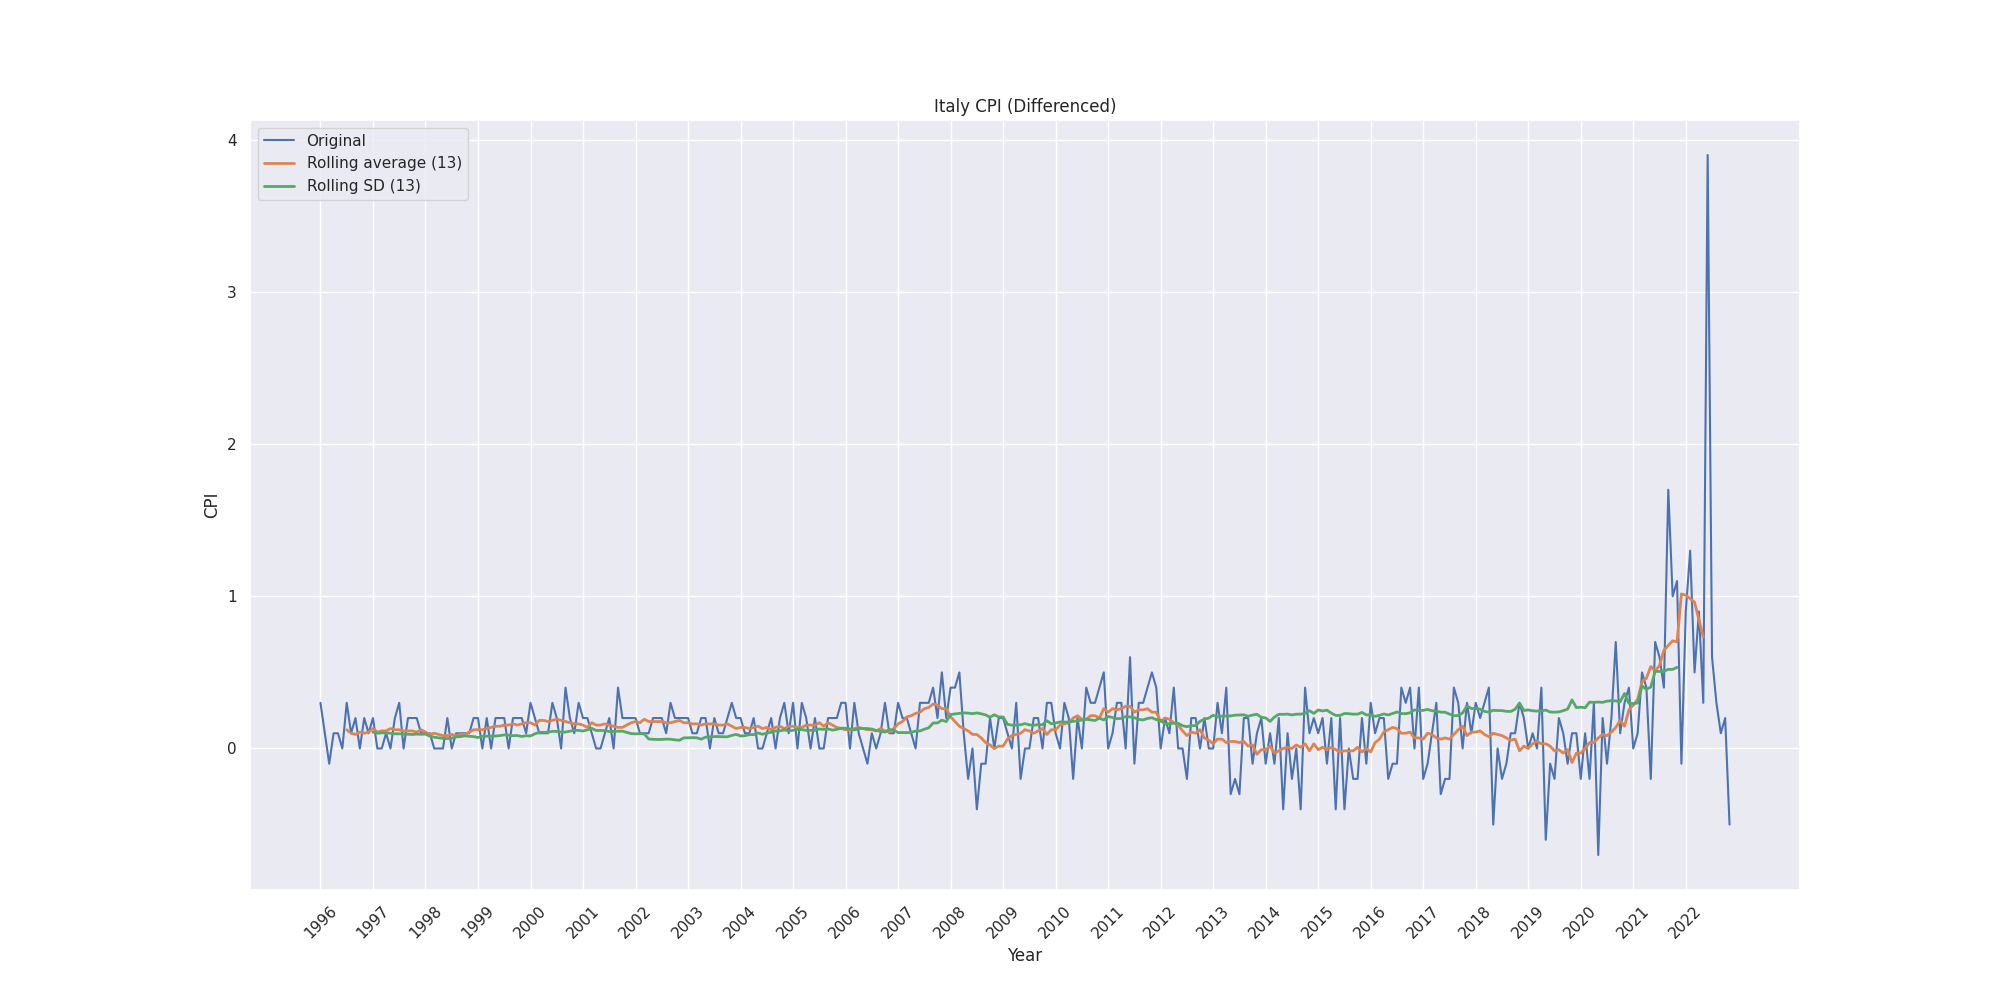
\includegraphics[width=.9\linewidth]{imgs/italy_cpi_diff.png}
  \caption{Time series first differences for Italy}
  \label{fig:italy_diff}
\end{figure}

The algorithm is shown in the following pseudo-code:
\begin{lstlisting}[language=Python]
def fit(x,y):
  model = OLS(y,x).fit()
  rho = compute_rho(model)
  while not convergence_criteria:
      model = prais_winsten(model, rho)
      rho = compute_rho(model)
  return model, rho

def compute_rho(model):
  e_0 = model.resid[1:]
  e_1 = model.resid[:-1]
  return np.dot(e_1,e_0)/np.dot(e_1,e_1)

def prais_winsten(self, model, rho):
  x_0 = np.sqrt(1 - rho**2) * x[0]
  y_0 = np.sqrt(1 - rho**2) * y[0]
  x_t = x[1:,] - rho * x[:-1,]
  y_t= y[1:] - rho * y[:-1]
  x = np.append(x_0, x_t, axis=0)
  y = np.append(y_0, y_t)
  return OLS(y, x).fit()
\end{lstlisting}

\subsection*{Results}
We then apply the Prais-Winsten Estimator to the differenced data. The results of the regression are shown in Table \ref{tab:italy_pw}. As we can see the results are inconclusive, as the R-squared is very low and the p-value is only significant for the Interest Rate variable. Moreover the coefficients are very close to zero, which probably implies that the model is not a good fit for the data.

\begin{center}
    {\small
  \begin{tabular}{cccccc}
                             & \textbf{coef} & \textbf{std err} & \textbf{t} & \textbf{P$> |$t$|$} & \textbf{[0.025 0.975]} \\
    \hline    \textbf{const} & 0.0009        & 0.009            & 0.096      & 0.924               & [-0.017 0.019 ]        \\
    \textbf{ir}              & -0.0080       & 0.003            & -2.561     & 0.011               & [-0.014 -0.002]        \\
    \textbf{cpi}             & -0.0020       & 0.001            & -1.659     & 0.098               & [-0.004 0.000 ]        \\
    \hline
  \end{tabular}
  }
  \begin{tabular}{lc}
    Statistics                              &        \\
    \hline
    \textbf{  R-squared (uncentered):}      & 0.042  \\
    \textbf{  Adj. R-squared (uncentered):} & 0.031  \\
    \textbf{  F-statistic:       }          & 3.605  \\
    \textbf{  Prob (F-statistic):}          & 0.0141 \\
    \textbf{  Log-Likelihood:    }          & 900.71 \\
    \textbf{  AIC:               }          & -1795. \\
    \textbf{  BIC:               }          & -1785. \\
    \textbf{No. Observations:}              & 248    \\
    \textbf{Df Residuals:}                  & 245    \\
    \hline
  \end{tabular}
  \label{tab:italy_pw}
\end{center}


In the regression's diagnostic plots in Figure \ref{fig:italy_diag} we can see in the residuals vs fitted plot that the residuals can be considered white noise and the QQ plot is acceptable to suggest normality. However, even if all these plots don't seem to show any major issue, the low R-squared and the non-significant p-values suggest that the model is not a good fit for the data anyway.
\begin{figure}[H]
  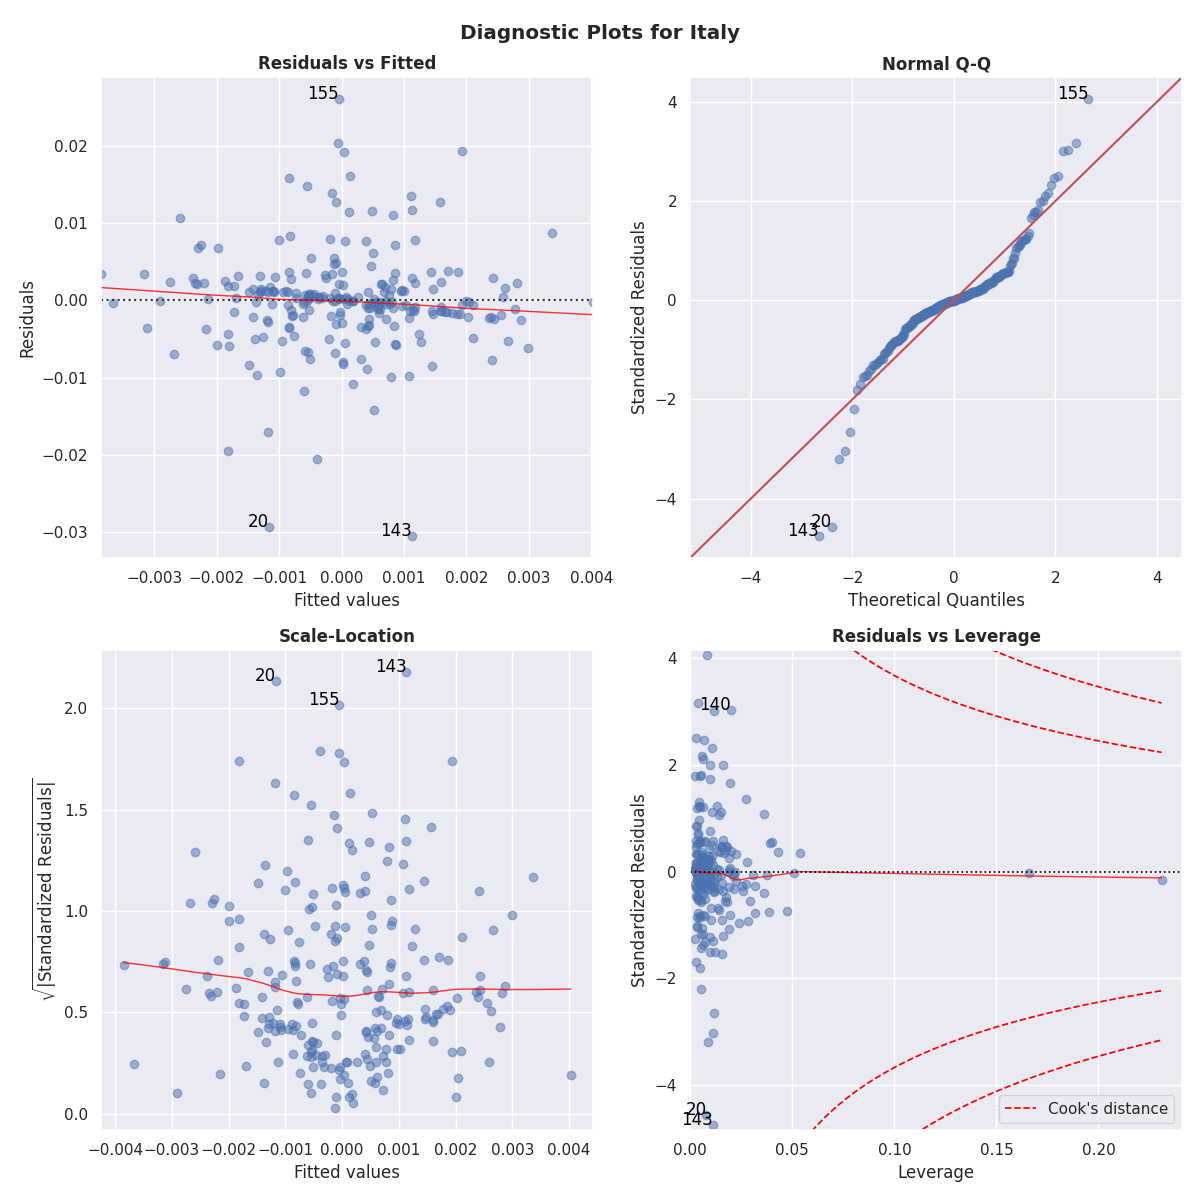
\includegraphics[width=.9\linewidth]{imgs/italy_diagnostic_plots.png}
  \caption{Diagnostic plots for Italy}
  \label{fig:italy_diag}
\end{figure}

This lack of fit can be further confirmed by predicting the future values of GDP using the model both for the test set and for the COVID data. We can see that the prediction is roughly constant but more importantly the prediction intervals are extremely wide, which means that the model is not able to predict the future values of GDP with any degree of certainty (Figure \ref{fig:italy_pw_pred}).
The prediction intervals are computed according to this paper \cite{prais_ci}
\begin{align*}
  \hat{Y_t} \pm t_{1-\alpha/2, n-2} \eta_n
  \eta_n = \hat{\sigma} \left( \frac{\sum_{i=1}^n(X_i - X_t)^2}{n \sum_{i=1}^n (X_i - \bar{X})} + \frac{1}{1-\hat{\rho}^2} \right)
\end{align*}

Moreover, it is interesting to note the chart of the one-step ahead predictions, which uses the true values of GDP up to time step $t-1$ to predict exclusively the value at time step $t$. This graph is satisfactory, as the predictions are very close to the true values, but the task is much simpler since only one step is predicted.
\begin{figure}[H]
  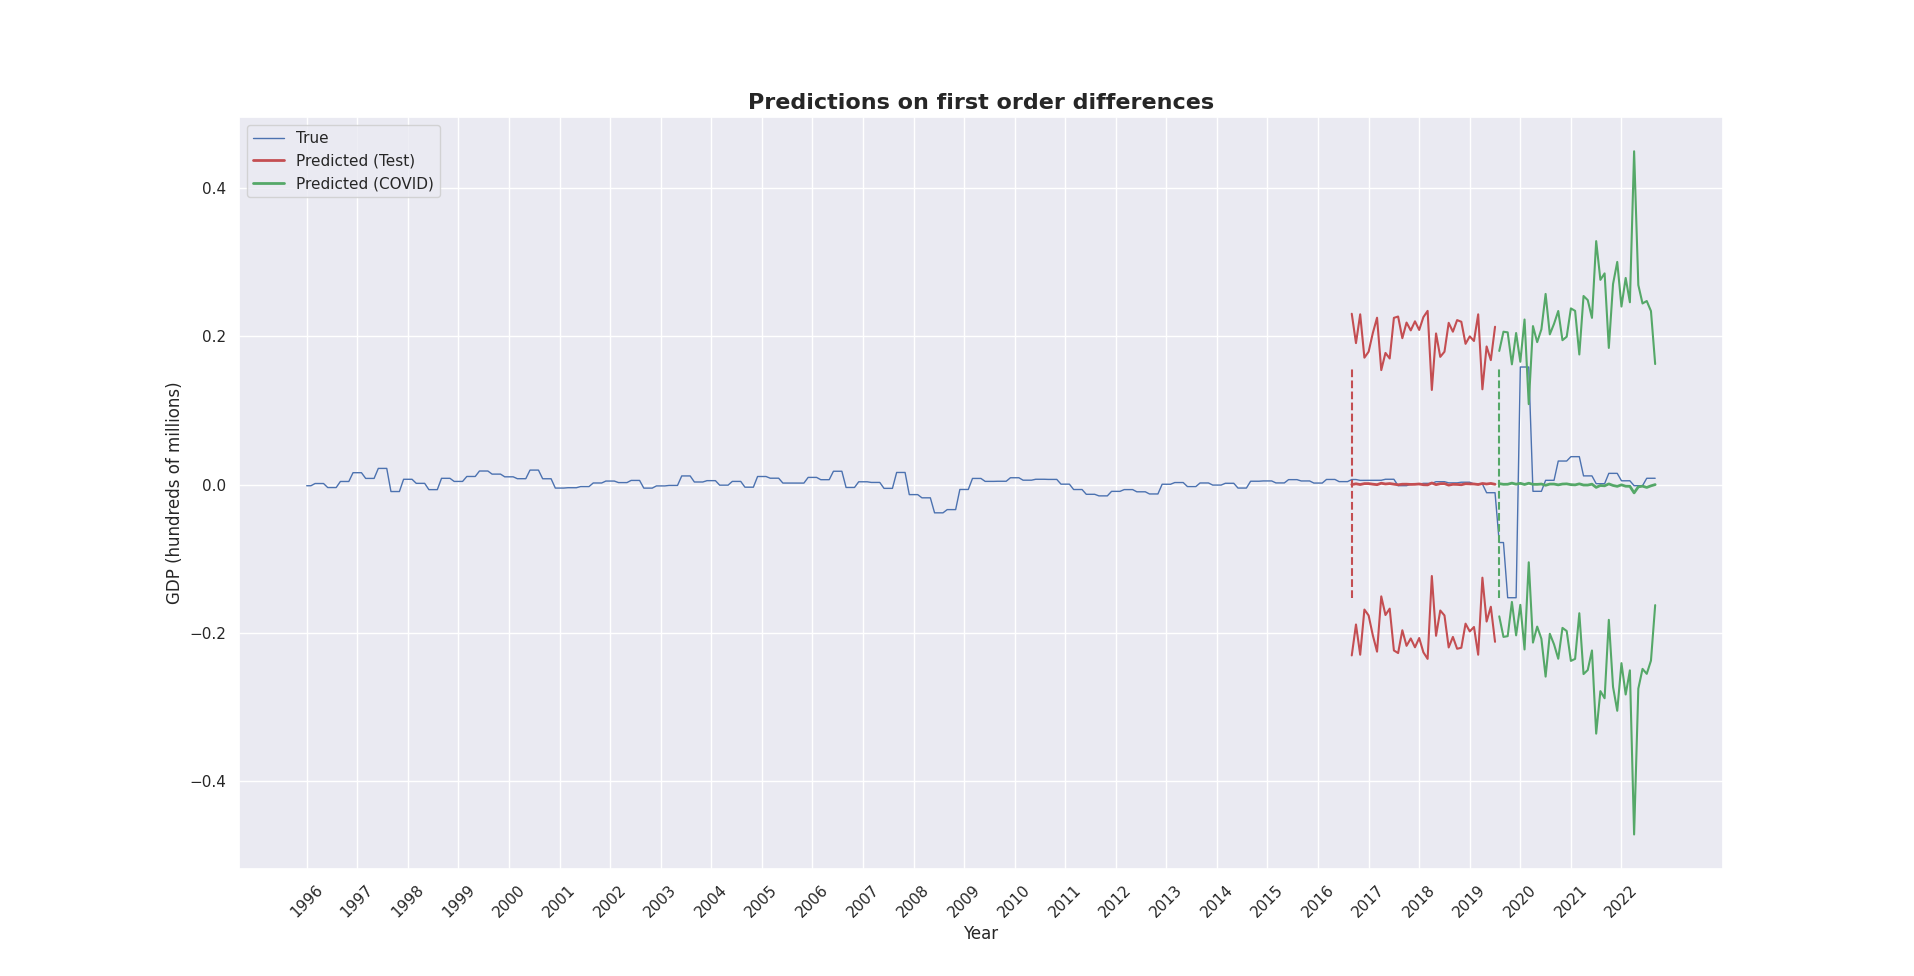
\includegraphics[width=.9\linewidth]{imgs/italy_pred_diff.png}
  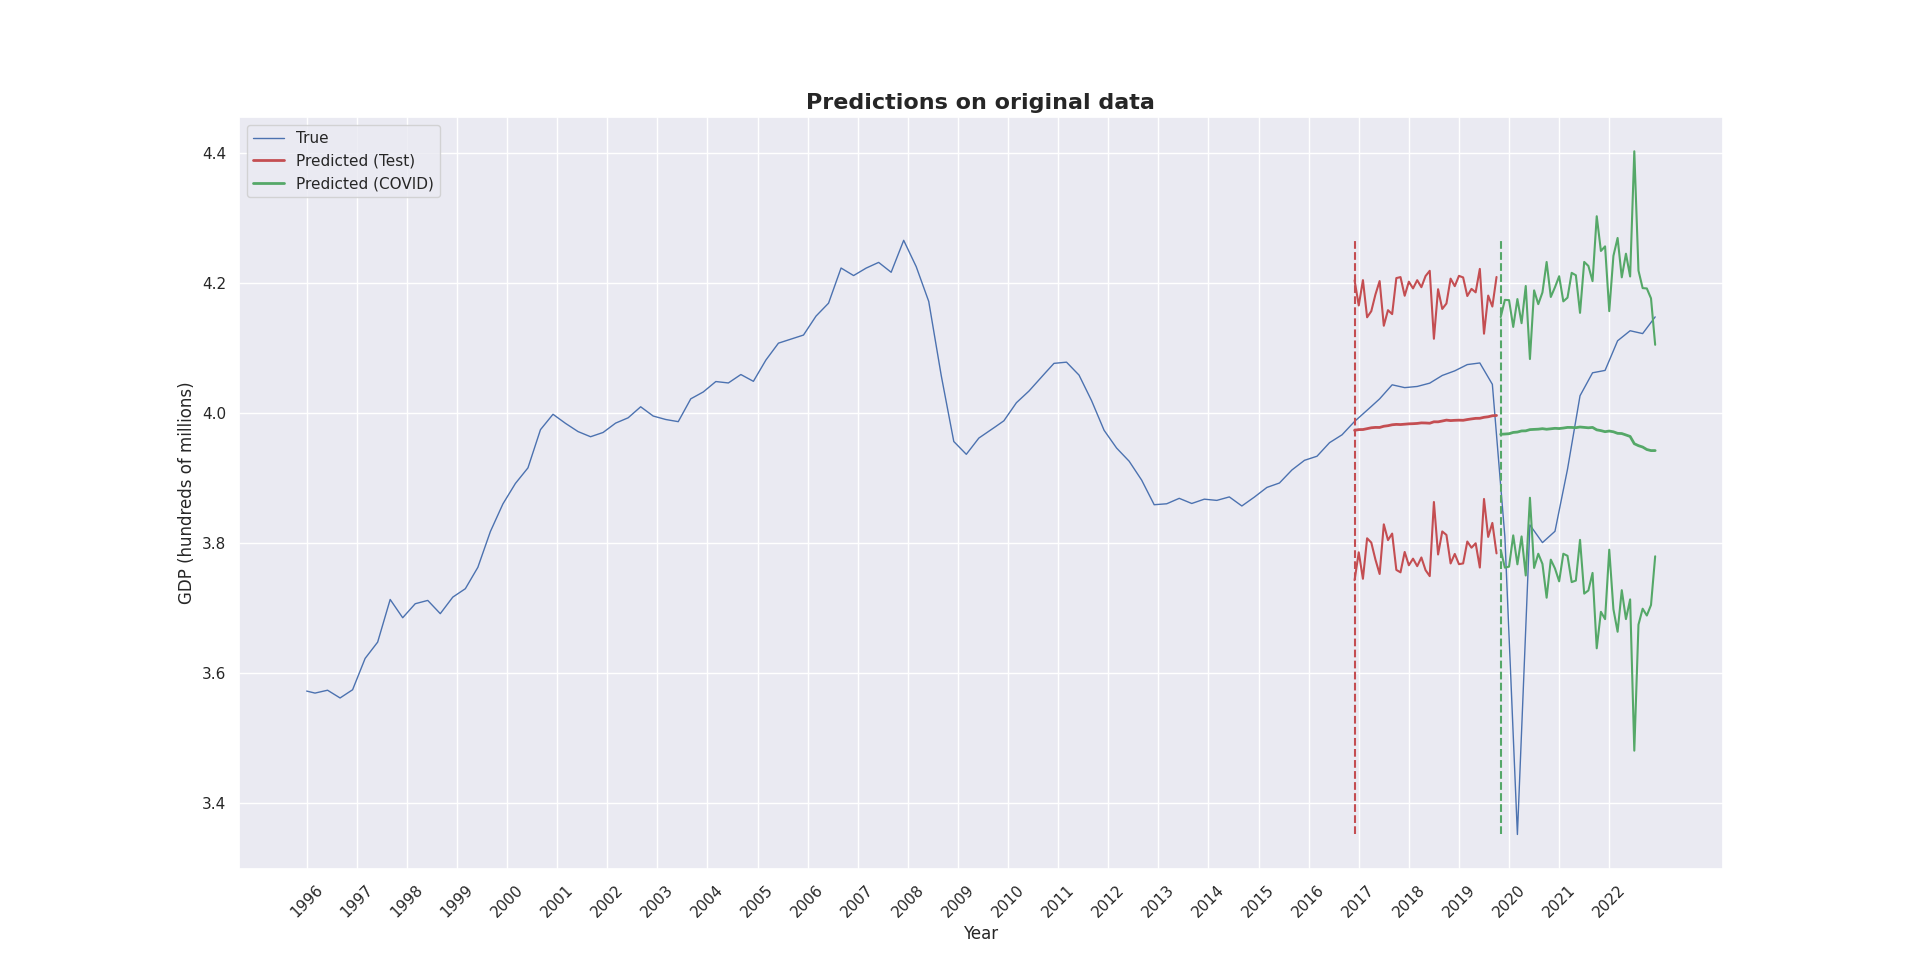
\includegraphics[width=.9\linewidth]{imgs/italy_reg_predictions.png}
  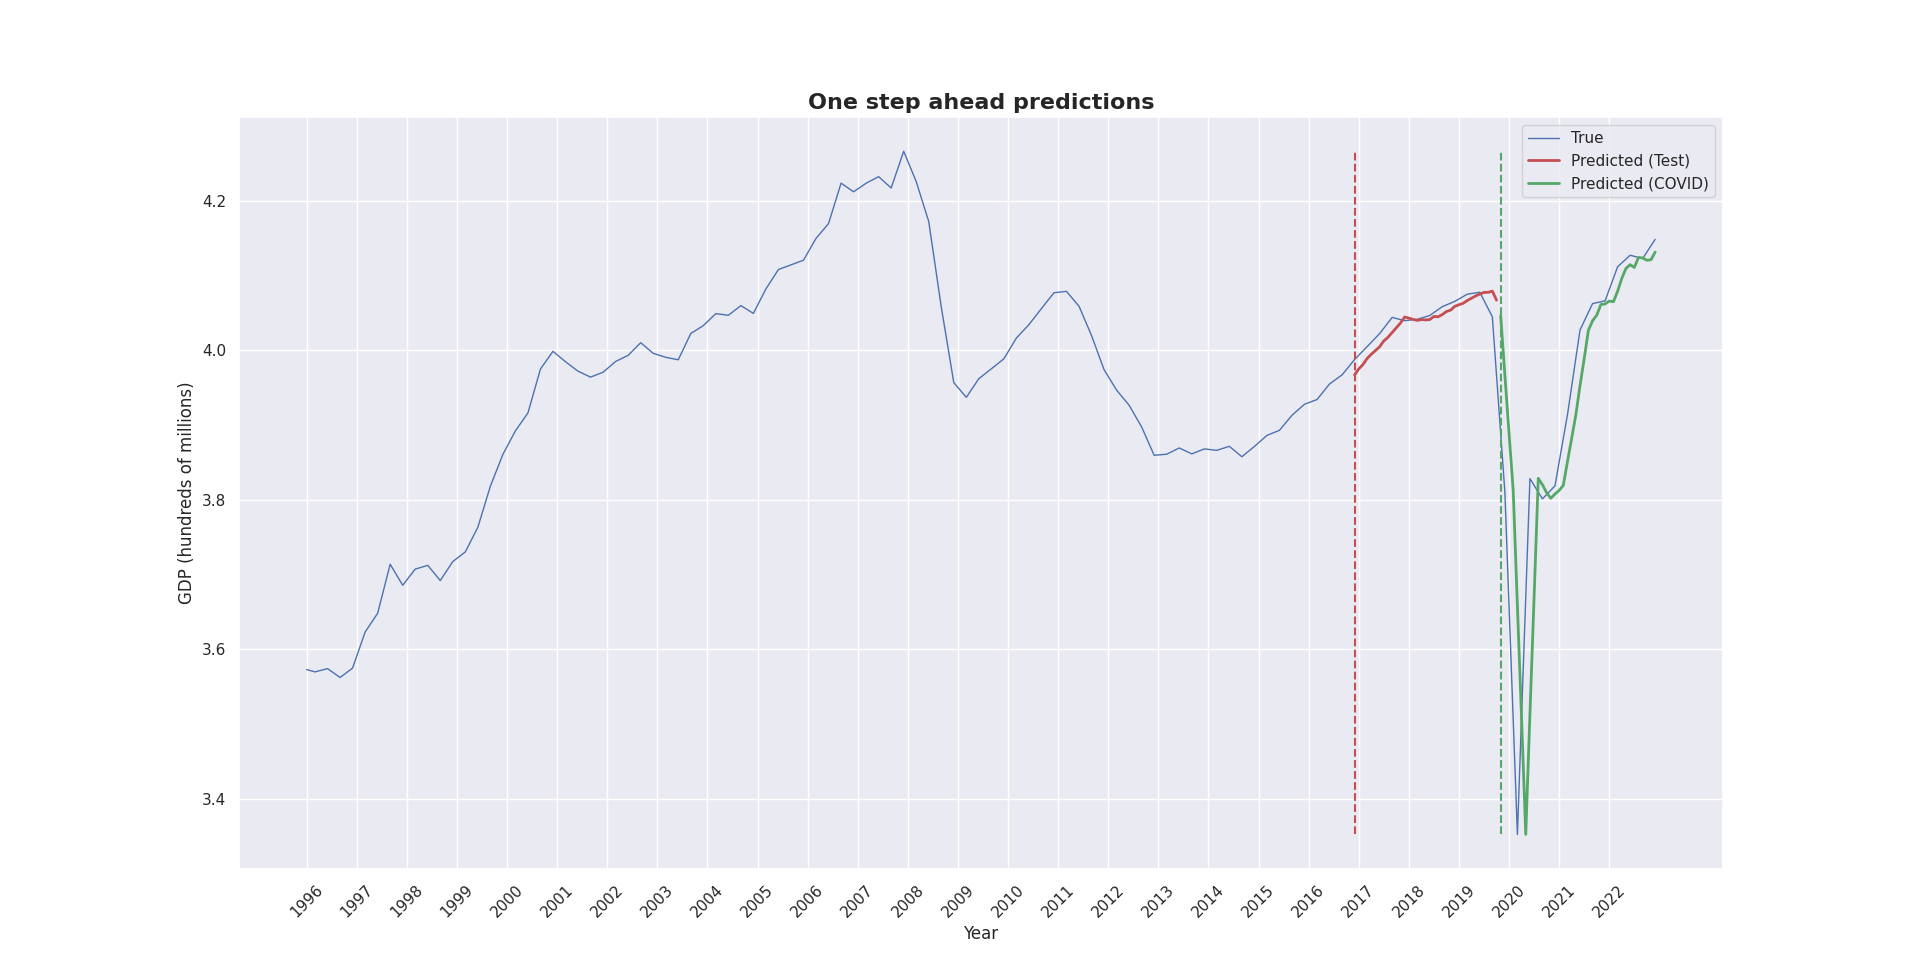
\includegraphics[width=.9\linewidth]{imgs/italy_pred_one_ahead.png}
  \caption{Prais-Winsten Estimator predictions for Italy}
  \label{fig:italy_pw_pred}
\end{figure}

The most probable reason for the poor performance of the model is that the assumption that the residuals are modelled by an $AR(1)$ process is very simplistic and does not capture the complexity of the data. By observing the ACF and PACF of the residuals (Figure \ref{fig:italy_res_corr}) we can see that the residuals are not well modelled by an $AR(1)$ process, as there are several lags that are significant and the ACF does not decay quickly. This implies that the residuals are not white noise and the model is not a good fit for the data. A possible improvement that could be done is to try a more complex model for the residuals; given that both the autocorrelation and the partial autocorrelation exhibit a sinusoidal pattern an ARMA model could be considered \cite{ts_intro}pg.356.
\begin{figure}[H]
  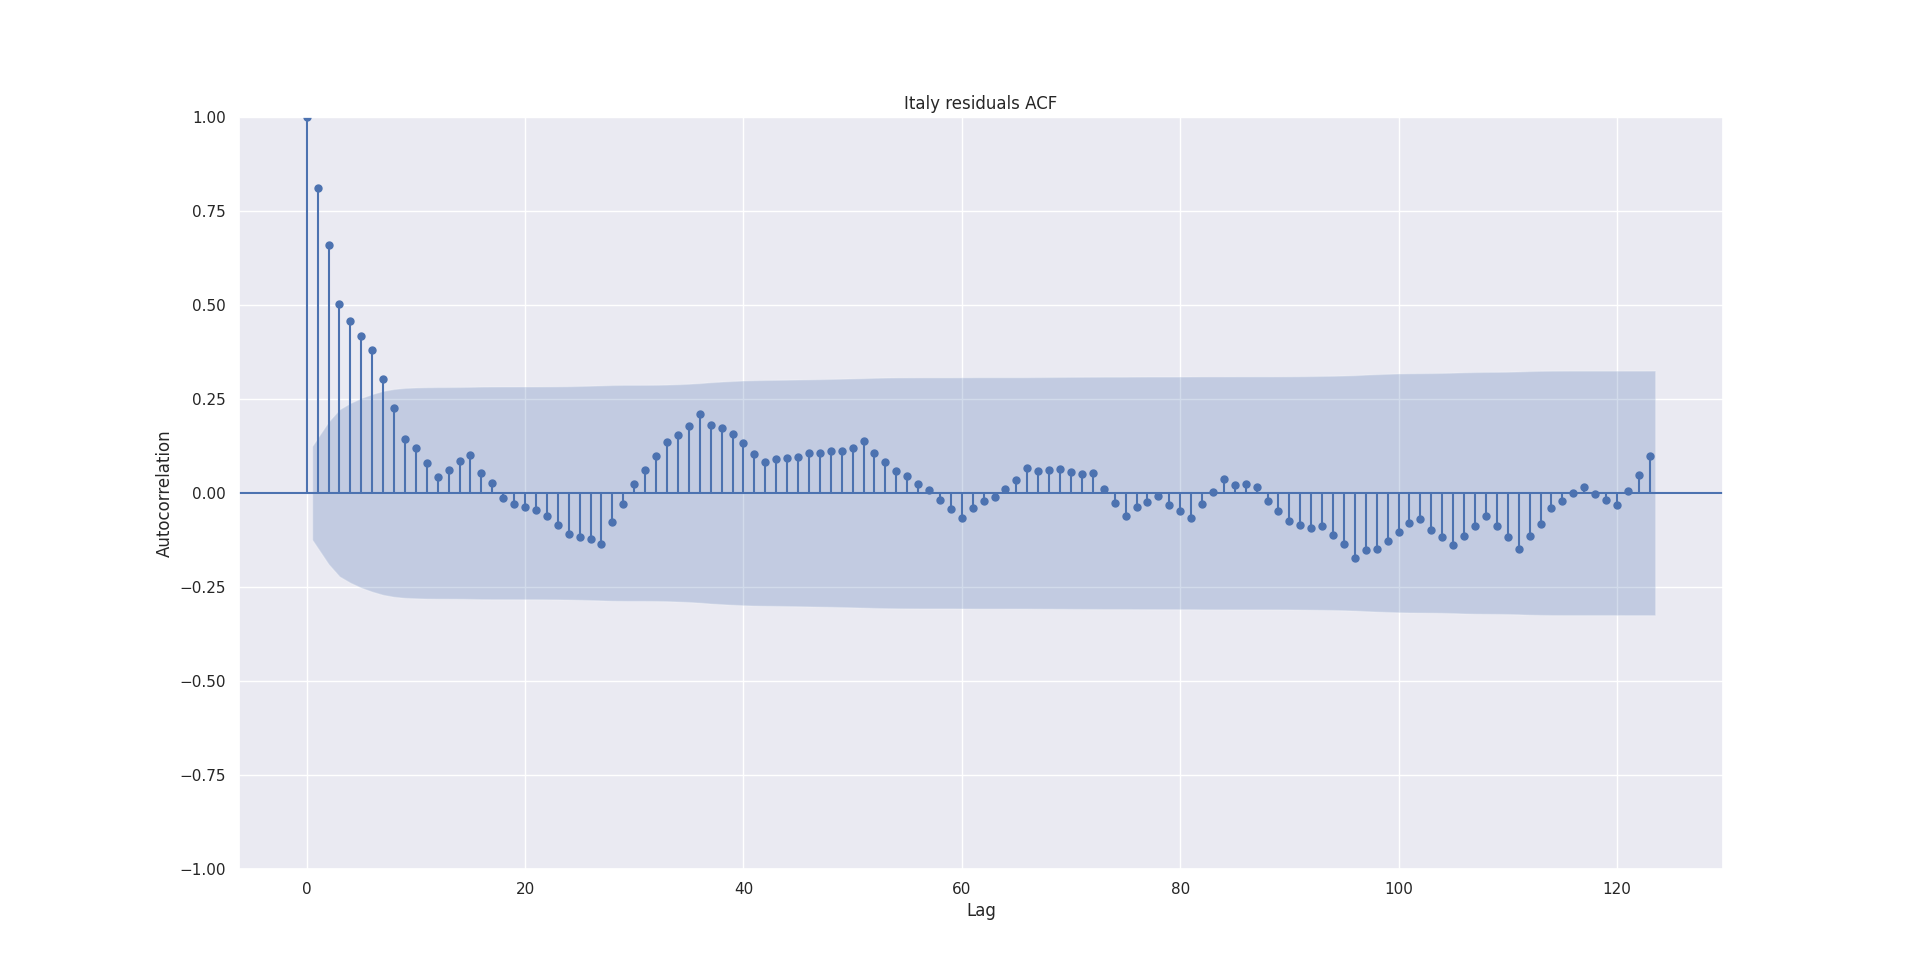
\includegraphics[width=.9\linewidth]{imgs/italy_res_acf.png}
  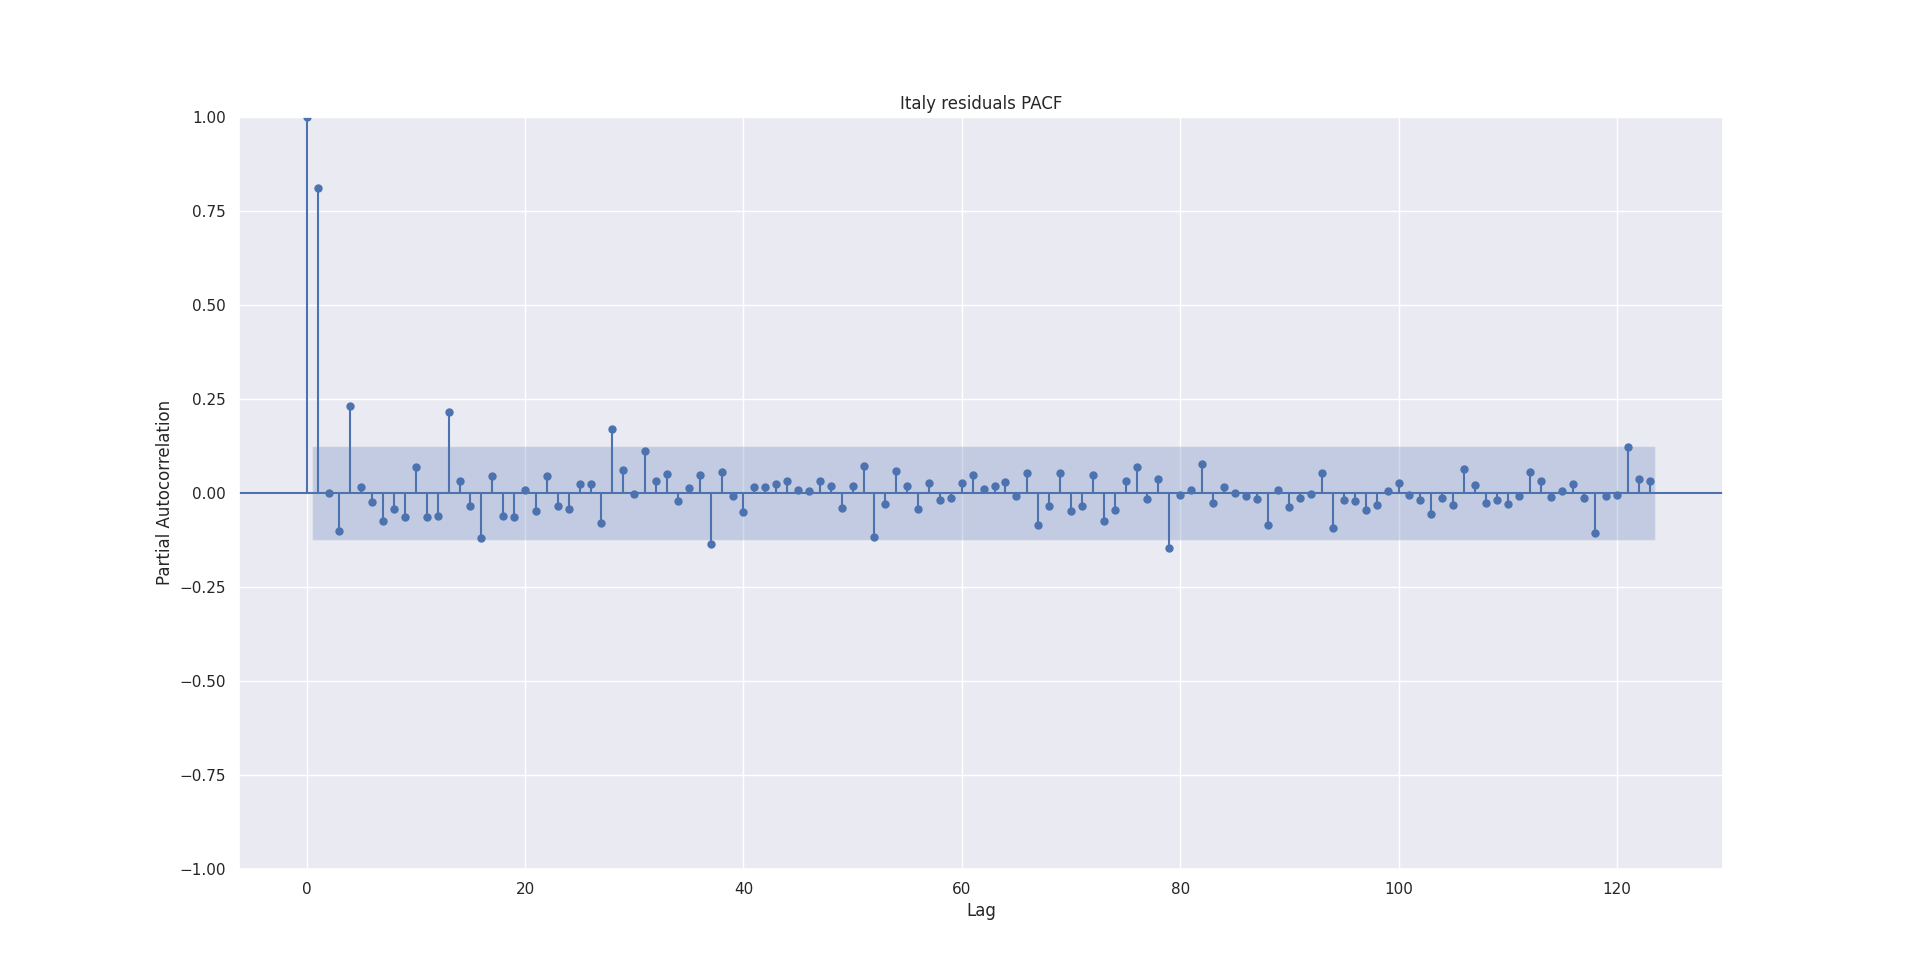
\includegraphics[width=.9\linewidth]{imgs/italy_res_pacf.png}
  \caption{Residuals ACF and PACF for Italy}
  \label{fig:italy_res_corr}
\end{figure}

Another, more straightforward, improvement could be to include more variables in the regression, as the model is extremely limited with only two variables.

\section{HIDDEN MARKOV MODEL PREDICTION}
\label{sec:hmm}
We can try a different method to predict the future of an economy. We can study the economies as a Markov Chain, a stochastic model describing a sequence of possible events in which the probability of each event depends only on the state attained in the previous event.

Our new approach involves incorporating three variables into a Hidden Markov Model. This version is designed to estimate the probabilities of transitioning from one state to another, relying not on direct knowledge of these probabilities but on observations of a related variable. To achieve this, we defined four basic states based on the possible increases and decreases in the Interest Rate and Consumer Price Index. Additionally, we considered two observable variables: the increase and decrease of GDP.

We will make some assumptions on the economic data, considering them dependent only on the previous point and not on the full sequence before them, and limiting the states only on positive or negative increases. The first assumption simplifies our work and allows us to use a Markov Chain, even if of course the complex relation of real economy figures is not so simple; the second does not capture the full spectrum of possibilities but allows us to more easily make consideration on the result, having only four states and two known variables. In the future, dividing the data into multiple steps could result in a better model that is able to differentiate between good and extreme differences: inflation at 3\% versus 80\% like in Türkiye; increasing the interest rate from a base of -0.5\% versus from 4.5\%; a good increase of 4\% of GDP versus a 0.2\% increase that saves a country for being in a technical recession. For the scope of this paper, however, we will stick to the simpler version.

To create our model, we used the Baum-Welch Algorithm \cite{baum}. This algorithm is an iterative procedure that estimates the parameters of a Hidden Markov Model. We start with a Hidden Markov Chain and a known variable chain created from the statistics of one starting country and then we use the temporal series of all the country we have to improve our model over multiple iterations.

Based on the data available, we ended up using twenty-five countries: Brazil, Canada, Chile, Denmark, Finland, France, Germany, Greece, Ireland, India, Indonesia, Italy, Israel, Japan, Mexico, Netherlands, Norway, Russia, South Africa, Spain, Switzerland, South Korea, Ukraine, United Kingdom, United States. We divided the data so that recent measurements between 2017 and 2020 were used for testing, while after 2020 we make some considerations about the recent crisis. Not all countries used for training, however, have data available for the testing or COVID analysis, but they are still useful for the model iterations.

\subsection*{Baum Welch Algorithm}
We start by creating a starting HMM model by calculating the probabilities from the starting country based on its data. We can define

\begin{itemize}
    \item $X_t$ as the hidden state at time $t$ (which can be a combination of increase/decrease of interest rate/consumer price index)
    \item $Y_t$ as the country observation temporal series of the known variable at time $t$ (which can be the increase or decrease of the GDP)
    \item $ A= \{a_{ij}\} = P(X_t = j | X_{t-1} = i)$ as the transition matrix between the hidden chain states
    \item $B = \{b_j(y_i)\} = P(Y_t = y_i | X_t = j)$ as the observation matrix between a a known variable and hidden state
    \item$\pi$ as the initial hidden state distribution
\end{itemize}
We will call the Hidden Markov chain \(\theta = (A,B,\pi)\).

Then, we iterate for the number of epochs by calculating for each country temporal series the forward ($\alpha$) and backward ($\beta$) probabilities, where

\[\alpha_t(i) = P(Y_1 = y_1, ..., Y_t = y_t, X_t = i | \theta)\]

are the probabilities of seeing the observations $y_1, ..., y_t$ and being in state $i$ at time $t$, calculated as

\[\alpha_i(1) = \pi_i b_i(y_1)\]
\[\alpha_i(t+1) = b_i(y_{t+1}) \sum_{j=1}^{N} \alpha_j(t) a_{ji}\]

and

\[\beta_t(i) = P(Y_{t+1} = y_{t+1}, ..., Y_T = y_T | X_t = i, \theta)\]

are the probabilities of the ending partial sequence $y_{t+1}, ..., y_T$ given starting state $i$ at time $t$, calculated as

\[\beta_i(T) = 1\]
\[\beta_i(t) = \sum_{j=1}^{N} a_{ij} b_j(y_{t+1}) \beta_j(t+1)\]

We can calculate the temporary variables

\[\gamma_t(i) = P(X_t = i | Y, \theta) = \frac{\alpha_i(t)\beta_i(t)}{\sum_{j=1}^{N} \alpha_j(t) \beta_j(t)}\]

being the probability of being in state $i$ at time $t$

\[\xi_t(i, j) = P(X_t = i, X_{t+1} = j | Y, \theta) =\]

\[\frac{\alpha_i(t) a_{ij} \beta_j(t+1) b_j(y_t+1)}{\sum_{k=1}^{N}\sum_{w=1}^{N}\alpha_k(t) a_{kw} \beta_w(t+1) b_w(y_t+1)}\]

being the probability of transitioning from state $i$ to state $j$ at time $t$

If we calculate $(\alpha_r, \beta_r, \gamma_r, \xi_r)$ $\forall r \in R \text{ countries }$, we can use all of them to update the parameters of $\theta$

\[\pi_i = \sum_{r=1}^{R} \gamma_{ir}(1)\]

\[a_{ij} = \frac{\sum_{r=1}^{R} \sum_{t=1}^{T-1} \xi_{ijr}(t)}{\sum_{r=1}^{R} \sum_{t=1}^{T-1} \gamma_{ir}(t)}\]

\[b_i(v_k) = \frac{\sum_{r=1}^{R} \sum_{t=1}^{T} 1_{y_{tr} \ne v_k} \gamma_{ir}(t)}{\sum_{r=1}^{R} \sum_{t=1}^{T} \gamma_{ir}(t)}\]

\[\text{where } 1_{y_{tr} \ne v_k} = \begin{cases} 1 & \text{if $y_{tr} \ne v_k$} \\ 0 & \text{otherwise} \end{cases}\]

\subsection*{Results}

By having now a model that can estimate the probabilities of transitioning from one state to another, we can use it to predict the future of a country. We must first test the model working on real data: to do that, we use the model trained on data until the end of 2016 and test it on data by making a thousand random walks and comparing results from the start of 2017 to the end of 2019. We can then do the same, only this time with the covid data from the start of 2020 onward to see if the model deviates and how much. Here we show some results on some countries, Italy and United States.

% substitute ± with (@$\pm$@)

\subsubsection*{Italy}

We can see here that the model is able to predict the future of Italy quite well, with the average of the known states being very close to the actual data. For the covid data, the real performance is a bit lower (27 versus predicted 32.37): even if it is inside the prediction interval, we can see how much the recent crisis have impacted the economy.

\begin{figure}[H]
    \centering
    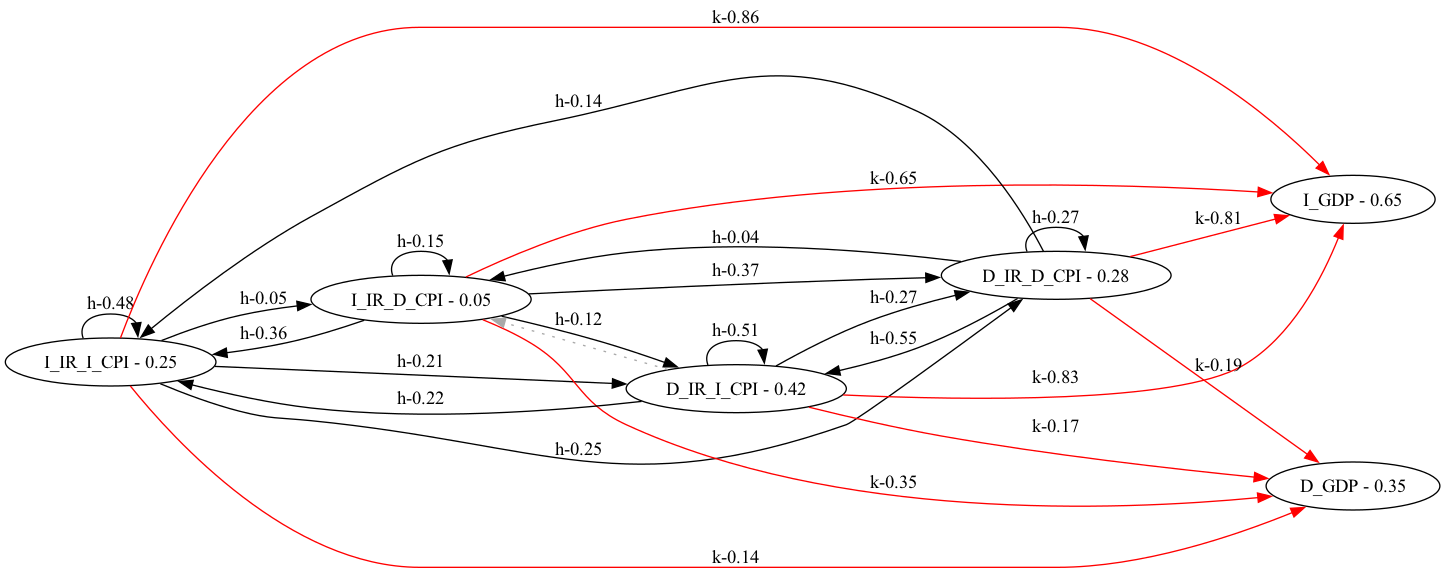
\includegraphics[width=\columnwidth]{imgs/italy_hmm.png}
    \caption{Hidden Markov Chain for Italy}
    \label{fig:correlation_us}
\end{figure}

\begin{table}[H]
  \centering
  \begin{tabular}{|c|c|c|c|}
    \hline
    State         & Ground Truth & Prediction & PI     \\
    \hline
    I\_IR\_I\_CPI & 8            & 9.95       & ± 7.20 \\
    I\_IR\_D\_CPI & 2            & 1.02       & ± 2.19 \\
    D\_IR\_I\_CPI & 11           & 15.57      & ± 7.21 \\
    D\_IR\_D\_CPI & 15           & 9.46       & ± 5.26 \\
    I\_GDP        & 30           & 29.85      & ± 4.38 \\
    D\_GDP        & 6            & 6.15       & ± 4.38 \\
    \hline
  \end{tabular}
  \label{tab:italy_test}
  \caption{Hidden Markov Model predictions for test set of Italy}
\end{table}

\begin{table}[H]
  \centering
  \begin{tabular}{|c|c|c|c|}
    \hline
    State         & Ground Truth & Prediction & PI     \\
    \hline
    I\_IR\_I\_CPI & 13           & 10.80      & ± 6.99 \\
    I\_IR\_D\_CPI & 3            & 1.11       & ± 2.29 \\
    D\_IR\_I\_CPI & 14           & 16.75      & ± 7.12 \\
    D\_IR\_D\_CPI & 9            & 10.34      & ± 5.54 \\
    I\_GDP        & 27           & 32.37      & ± 4.49 \\
    D\_GDP        & 12           & 6.63       & ± 4.49 \\
    \hline
  \end{tabular}
  \label{tab:italy_covid}
  \caption{Hidden Markov Model predictions for covid data of Italy}
\end{table}

\subsubsection*{United States}

The United States, like before, are quite the outliers: since the model is trained on all countries even if the USA have not experienced a single month of negative GDP growth, the prediction is a bit more pessimistic (even if it is still inside our prediction interval). The situation during the COVID pandemic changes things: during this negative period, the USA mighty performance is similar to a normal country before the crisis.

\begin{figure}[H]
    \centering
    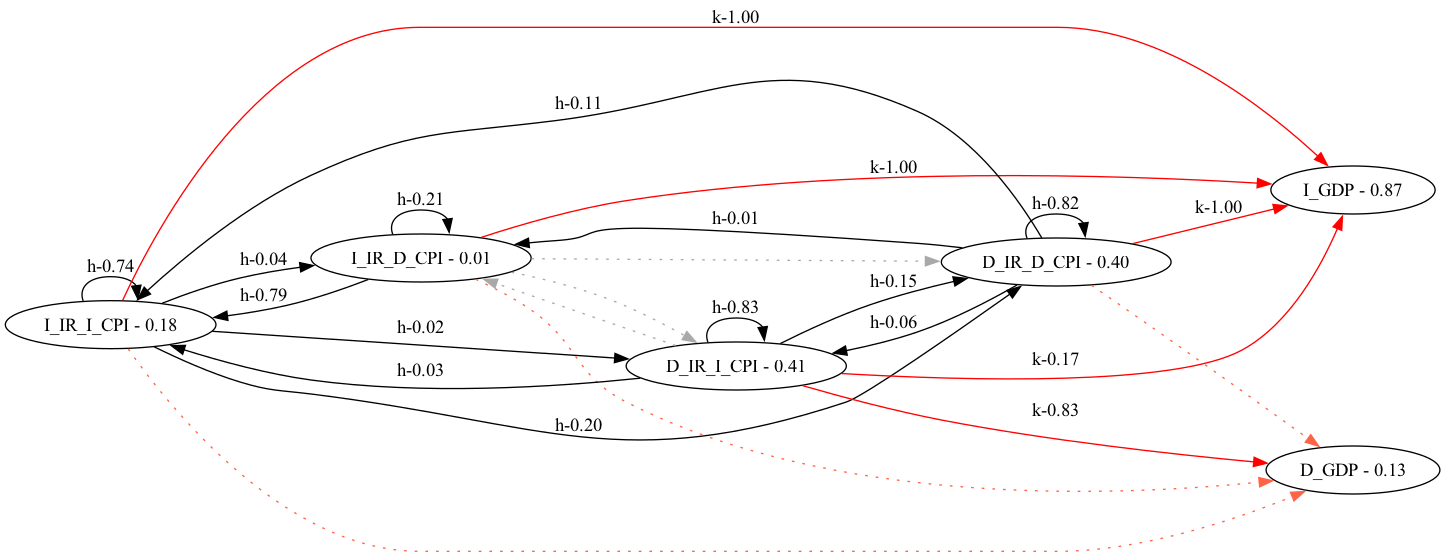
\includegraphics[width=\linewidth]{imgs/usa_hmm.png}
    \caption{Hidden Markov Chain for USA}
    \label{fig:correlation_us}
\end{figure}

\begin{table}[H]
  \centering
  \begin{tabular}{|c|c|c|c|}
    \hline
    State         & Ground Truth & Prediction & PI      \\
    \hline
    I\_IR\_I\_CPI & 10           & 10.47      & ± 11.57 \\
    I\_IR\_D\_CPI & 2            & 0.75       & ± 2.21  \\
    D\_IR\_I\_CPI & 2            & 7.23       & ± 12.30 \\
    D\_IR\_D\_CPI & 22           & 17.55      & ± 12.40 \\
    I\_GDP        & 36           & 29.93      & ± 10.34 \\
    D\_GDP        & 0            & 6.07       & ± 10.34 \\
    \hline
  \end{tabular}
  \label{tab:usa_test}
  \caption{Hidden Markov Model predictions for test set for USA}
\end{table}

\begin{table}[H]
  \centering
  \begin{tabular}{|c|c|c|c|}
    \hline
    State         & Ground Truth & Prediction & PI     \\
    \hline
    I\_IR\_I\_CPI & 0            & 5.93       & ± 8.63 \\
    I\_IR\_D\_CPI & 0            & 0.40       & ± 1.58 \\
    D\_IR\_I\_CPI & 0            & 3.73       & ± 8.66 \\
    D\_IR\_D\_CPI & 20           & 9.95       & ± 9.10 \\
    I\_GDP        & 14           & 16.85      & ± 7.37 \\
    D\_GDP        & 6            & 3.15       & ± 7.37 \\
    \hline
  \end{tabular}
  \label{tab:usa_covid}
  \caption{Hidden Markov Model predictions for covid data for USA}
\end{table}

\subsubsection*{South Korea}
With South Korea the testing of our prediction is well acceptable. The test on the covid data however is also quite similar: the republic of Korea had an excellent mechanism of contact tracing and random tests on the population, resulting in a better management of the pandemic, suffered much less than other countries and that resulted in an economy that was not as damaged as the others.

\begin{figure}[H]
    \centering
    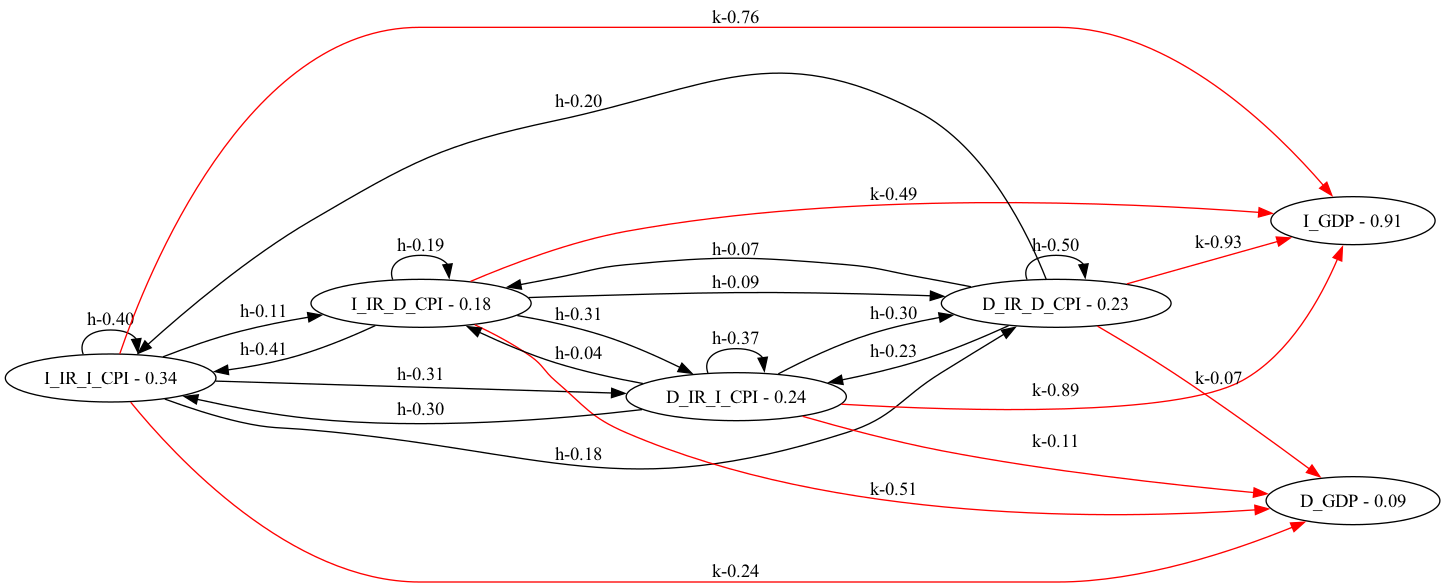
\includegraphics[width=\linewidth]{imgs/sk_hmm.png}
    \caption{Hidden Markov Chain for South Korea}
    \label{fig:correlation_sk}
\end{figure}

\begin{table}[H]
  \centering
  \begin{tabular}{|c|c|c|c|}
    \hline
    State         & Ground Truth & Prediction & PI      \\
    \hline
    I\_IR\_I\_CPI & 8           & 11.07 & ± 6.19 \\
    I\_IR\_D\_CPI & 6            & 2.98 & ± 3.59  \\
    D\_IR\_I\_CPI & 11            & 11.07 & ± 5.93 \\
    D\_IR\_D\_CPI & 11          & 10.88 & ± 7.01 \\
    I\_GDP        & 30           & 29.86 & ± 4.42 \\
    D\_GDP        & 6            & 6.14 & ± 4.42 \\
    \hline
  \end{tabular}
  \label{tab:sk_test}
  \caption{Hidden Markov Model predictions for test set for South Korea}
\end{table}

\begin{table}[H]
  \centering
  \begin{tabular}{|c|c|c|c|}
    \hline
    State         & Ground Truth & Prediction & PI     \\
    \hline
    I\_IR\_I\_CPI & 17            & 12.01 & ± 6.54 \\
    I\_IR\_D\_CPI & 4            & 3.22 & ± 3.93 \\
    D\_IR\_I\_CPI & 12            & 11.87 & ± 6.2 \\
    D\_IR\_D\_CPI & 6           & 11.90 & ± 7.40 \\
    I\_GDP        & 30           & 32.41 & ± 4.80 \\
    D\_GDP        & 9            & 6.58 & ± 4.80 \\
    \hline
  \end{tabular}
  \label{tab:sk_covid}
  \caption{Hidden Markov Model predictions for covid data for South Korea}
\end{table}

\subsubsection*{Model degeneration}
To train the HMM, we used 3 epochs: each time we improved our model on all temporal series, and then repeat. What would happen if we increased a lot the number of epochs? Let's try with 25 epochs.

\begin{figure}[H]
    \centering
    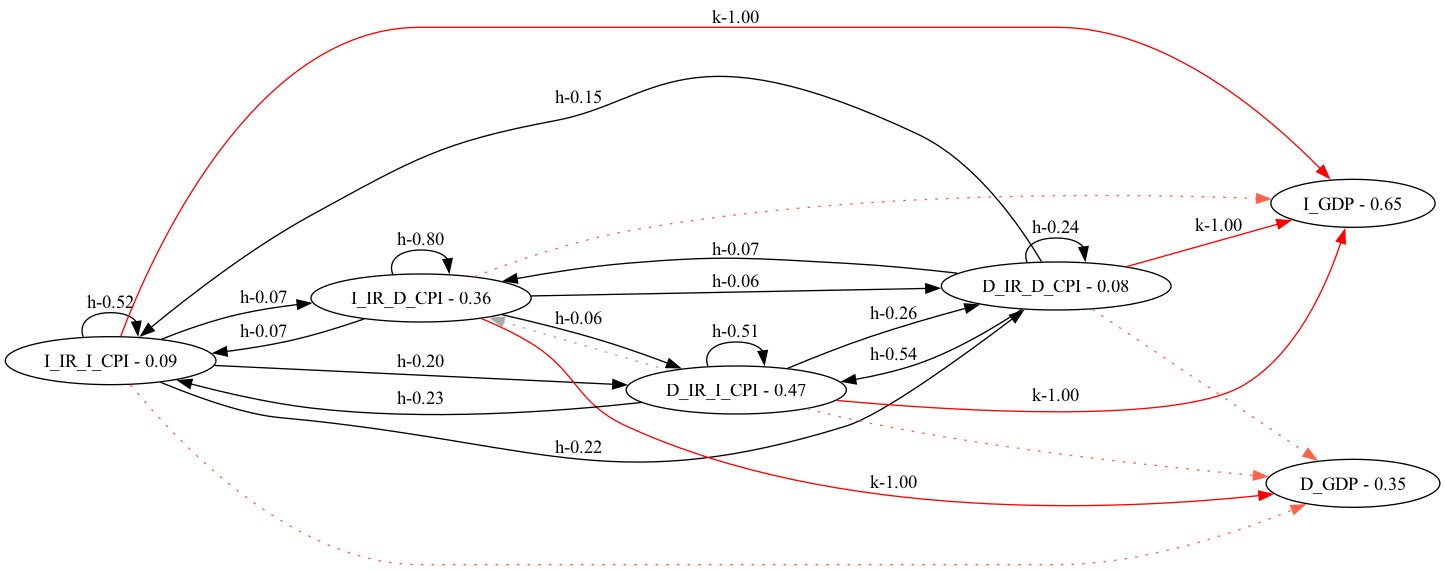
\includegraphics[width=\columnwidth]{imgs/italy_hmm_degenerated.png}
    \caption{Hidden Markov Chain for Italy (degenerated)}
    \label{fig:correlation_us}
\end{figure}

% \begin{lstlisting}
%   ITALY training data has 162 positive and 87 negative values for GDP ([ 66.00  8.00  108.00  67.00])

%   Use test data
%   ITALY testing data has 30 positive and 6 negative values for GDP ([ 8.00  2.00  11.00  15.00])

%   ITALY random walks has produced on average ['9.41 (@$\pm$@) 7.44', '6.09 (@$\pm$@) 11.39', '12.95 (@$\pm$@) 8.43', '7.55 (@$\pm$@) 5.48'] for the hidden states and ['29.91 (@$\pm$@) 11.39', '6.09 (@$\pm$@) 11.39'] for the known states
%   On average we have predicted 29.91 (@$\pm$@) 11.39 positive and 6.09 (@$\pm$@) 11.39 negative values for GDP

%   Use covid data
%   ITALY covid data has 27 positive and 12 negative values for GDP ([ 13.00  3.00  14.00  9.00])

%   ITALY random walks has produced on average ['10.53 (@$\pm$@) 7.86', '6.16 (@$\pm$@) 11.46', '14.11 (@$\pm$@) 8.96', '8.20 (@$\pm$@) 5.59'] for the hidden states and ['32.84 (@$\pm$@) 11.46', '6.16 (@$\pm$@) 11.46'] for the known states
%   On average we have predicted 32.84 (@$\pm$@) 11.46 positive and 6.16 (@$\pm$@) 11.46 negative values for GDP
% \end{lstlisting}
\begin{table}[H]
  \centering
  \begin{tabular}{|c|c|c|c|}
    \hline
    State         & Ground Truth & Prediction & PI      \\
    \hline
    I\_IR\_I\_CPI & 8            & 9.41       & ± 7.44  \\
    I\_IR\_D\_CPI & 2            & 6.09       & ± 11.39 \\
    D\_IR\_I\_CPI & 11           & 12.95      & ± 8.43  \\
    D\_IR\_D\_CPI & 15           & 7.55       & ± 5.48  \\
    I\_GDP        & 30           & 29.91      & ± 11.39 \\
    D\_GDP        & 6            & 6.09       & ± 11.39 \\
    \hline
  \end{tabular}
  \label{tab:italy_test_degen}
  \caption{Hidden Markov Model predictions for test set for Italy (more epochs)}
\end{table}

\begin{table}[H]
  \centering
  \begin{tabular}{|c|c|c|c|}
    \hline
    State         & Ground Truth & Prediction & PI      \\
    \hline
    I\_IR\_I\_CPI & 13           & 10.53      & ± 7.86  \\
    I\_IR\_D\_CPI & 3            & 6.16       & ± 11.46 \\
    D\_IR\_I\_CPI & 14           & 14.11      & ± 8.96  \\
    D\_IR\_D\_CPI & 9            & 8.20       & ± 5.59  \\
    I\_GDP        & 27           & 32.84      & ± 11.46 \\
    D\_GDP        & 12           & 6.16       & ± 11.46 \\
    \hline
  \end{tabular}
  \label{tab:italy_covid_degen}
  \caption{Hidden Markov Model predictions for covid data of Italy (more epochs)}
\end{table}
We can see how our prediction is still working. We have the same mean but larger prediction intervals: each random walk weights more now. The model has degenerated: each hidden state goes only to one known state. Since the testing still works, we could say that this Markov Chain is showing us a correlation. All states but I\_IR\_D\_CPI increases the GDP: an increase in the interest rate and a decrease in the inflation instead decreases it. This result is in line with our initial assumptions, although simplified.

We can also see some missing links that are quite logical, like from I\_IR\_D\_CPI to D\_IR\_I\_CPI, and most states but D\_IR\_D\_CPI tend to remain in the same state. This also makes sense: if the inflation is decreasing and we decrease the interest rate, the inflation is going to go up since people will start borrowing money more frequently.

\newpage
\section{CONCLUSIONS}

In this project, we aimed to investigate the correlation between GDP, interest rates, and inflation by examining historical economic data from leading economies. Our analysis wanted to validate the current economic theory that hypothesizes an inverse relationship between GDP growth and interest rates and a correlation between GDP and inflation.

\subsection*{Correlation Analysis}
Our findings indicate a significant correlation between GDP and inflation, supporting the hypothesis that higher inflation often helps GDP growth. This aligns with the economic theory that as economies expand, the increased demand for goods and services tends to drive prices up.

The relationship between GDP and interest rates appears to be more complex. While an inverse correlation was observed in some cases, the strength and consistency of this relationship varied across different countries and time periods. This suggests that while interest rates are a critical tool for managing economic growth, their impact on GDP is influenced by a multitude of factors.

\subsection*{Model Predictions}
Utilizing Hidden Markov Models (HMM) for predicting economic indicators yielded good results. The models performed reasonably well on historical data, with predictions closely matching the actual economic trends. The confidence intervals were sound, and we can safely say that our prediction, although simplified, worked reasonably well.

Using the same model, we managed to find an higher prediction for the country economy compared to the result caused by the pandemic and the energy crisis that followed. These events have disrupted the economies and the lives of billions of people around the world, and with a more fine tuned model that uses more steps than just positive / negative changes (as explained in the introduction of the Hidden Markov Model chapter \ref{sec:hmm}) we could have a more precise prediction of how much growth did the recent events slowed down.

\subsection*{Policy Implications}
By finding correlations between the three variables studied, in particular between Inflation and Interest Rate, we can support the current economic theory and highlight the importance of the monetary policies the Central Banks apply in order to stabilize the economies of their countries.

It is important for policy makers to accurately calculate how much to fine tune, to avoid going too far and damage what they are trying to protect. The more precise analysis we described above, together with more accurate and frequent data, could be a valid assistance in choosing the best course of action.



% \section*{Acknowledgment}
% The authors would like to thank...



% trigger a \newpage just before the given reference
% number - used to balance the columns on the last page
% adjust value as needed - may need to be readjusted if
% the document is modified later
%\IEEEtriggeratref{8}
% The "triggered" command can be changed if desired:
%\IEEEtriggercmd{\enlargethispage{-5in}}

\newpage
\bibliographystyle{IEEEtran}
\bibliography{references.bib}

\end{document}
